%Dokumentenklasse "scrbook" - Erweitert um den Verweis auf die Verzeichnisse und Texteigenschaften
\documentclass[chapterprefix=true, 12pt, a4paper, oneside, parskip=half, listof=totoc, bibliography=totoc, numbers=noendperiod]{scrbook}

% Ränder (Standard bottom ca. 52mm anbzüglich von ca. 4mm für die nach oben rechts gewanderte Seitenzahl)
%Anpassung der Seitenränder
\usepackage[bottom=48mm,left=25mm,right=25mm]{geometry}

% Ränder bei Bedarf zeigen
%\usepackage{showframe}

%Tweaks für scrbook
\usepackage{scrhack}

%Blindtext
\usepackage{blindtext}

% todo
\usepackage{todonotes}

%Erlaubt unteranderem Umbrücke captions
\usepackage{caption}
%Stichwortverzeichnis
\usepackage{imakeidx}
%Kompakte Listen
\usepackage{paralist}

%Zitate besser formatieren und darstellen
\usepackage{epigraph}

%Glossar, Stichworverzeichnis
\usepackage{acronym}
\renewcommand*{\acsfont}[1]{\textnormal{#1}}

%Anpassung von Kopf- und Fußzeile
%beinflusst die erste Seite des Kapitels
% Set header
% []: Pages with chapter titles
% {}: Pages without chapter titles
% Inner head

\renewcommand*\chapterpagestyle{fancy}
% neue Kopfzeilen mit fancypaket
\usepackage{fancyhdr} %Paket laden
\pagestyle{fancy} %eigener Seitenstil
\fancyhf{} %alle Kopf- und Fußzeilenfelder bereinigen
\fancyhead[L]{\nouppercase{\leftmark}} %Kopfzeile links
\fancyhead[C]{} %zentrierte Kopfzeile
\fancyhead[R]{Hochschlue Luzern T\&A} %Kopfzeile rechts
\renewcommand{\headrulewidth}{0.4pt} %obere Trennlinie
\fancyfoot[R]{\thepage} %Seitennummer
\fancyfoot[L]{Daniel Zimmermann} %Seitennummer
\renewcommand{\footrulewidth}{0.4pt} %untere Trennlinie
%\renewcommand{\chapterpagestyle}{scrheadings}
%Auskommentieren für die Verkleinerung des vertikalen Abstandes eines neuen Kapitels
\renewcommand*{\chapterheadstartvskip}{\vspace*{.25\baselineskip}}


%Zeilenabstand 1,5
\usepackage[onehalfspacing]{setspace}
%Verbesserte Darstellung der Buchstaben zueinander
\usepackage[stretch=10]{microtype}
%Deutsche Bezeichnungen für angezeigte Namen (z.B. Innhaltsverzeichnis etc.)
\usepackage[ngerman]{babel}
%Unterstützung von Umlauten und anderen Sonderzeichen (UTF-8)
\usepackage{lmodern}
\usepackage[utf8]{luainputenc}
\usepackage[T1]{fontenc}
\usepackage{amsmath}

%Einfachere Zitate
\usepackage{epigraph}
%Unterstützung der H positionierung (keine automatische Verschiebung eingefügter Elemente)
\usepackage{float} 

%Erlaubt Umbrüche innerhalb von Tabellen
\usepackage{tabularx}
%Erlaubt Seitenumbrüche mit Tabellen
\usepackage{longtable}

%Erlaubt die Darstellung von Sourcecode mit Highlighting
\usepackage{listings}

%Definierung eigener Farben bei nutzung eines selbst vergebene Namens
%\usepackage[table,xcdraw]{xcolor}

\usepackage{pdfpages}



%Vektorgrafiken
\usepackage{tikz}
%Grafiken (wie jpg, png, etc.)
\usepackage{graphicx}
%Grafiken von Text umlaufen lassen
\usepackage{wrapfig}

%Ermöglicht Verknüpfungen innerhalb des Dokumentes (e.g. for PDF), Links werden durch "hidelink" nicht explizit hervorgehoben
\usepackage[hidelinks,german]{hyperref}

%Einbindung und Verwaltung von Literaturverzeichnissen
\usepackage{csquotes} %wird von biber benötigt
\usepackage[style=alphabetic, backend=biber, bibencoding=ascii]{biblatex}
\addbibresource{references/references.bib}

%-------------------------------Zusätzliche Anpassungen und Modifikationen--------------------------------------------%

%Anpassung der Überschriften
\addtokomafont{disposition}{\rmfamily}

%Zusätzliche Farben
\definecolor{darkgreen}{RGB}{0,100,0}

%Umbenennungen
\renewcommand{\lstlistlistingname}{Quelltextverzeichnis}

%Pluszeichen in der Referenc beim zitieren ausblenden
\renewcommand*{\labelalphaothers}{}

%Anpassugen zur Quelltextdarstellung, kann bei Bedarf überschrieben werden (z.B. wenn unterschiedliche Sprachen zum Einsatz kommen)
\renewcommand{\lstlistingname}{Codeauszug}
\lstset{
	language=Java,
	numbers=left,
	columns=fullflexible,
	aboveskip=5pt,
	belowskip=10pt,
	basicstyle=\small\ttfamily,
	backgroundcolor=\color{black!5},
	commentstyle=\color{darkgreen},
	keywordstyle=\color{blue},
	stringstyle=\color{gray},
	showspaces=false,
	showstringspaces=false,
	showtabs=false,
	xleftmargin=16pt,
	xrightmargin=0pt,
	framesep=5pt,
	framerule=3pt,
	frame=leftline,
	rulecolor=\color{green},
	tabsize=2,
	breaklines=true,
	breakatwhitespace=true,
	prebreak={\mbox{$\hookleftarrow$}}
}


%%Titles - Uncomment one section of titles

%%Used for titleGraduation
\makeatletter

\newcommand*{\gradeType}[1]{\gdef\@gradeType{#1}}
\newcommand*{\firstExaminer}[1]{\gdef\@firstExaminer{#1}}
\newcommand*{\secondExaminer}[1]{\gdef\@secondExaminer{#1}}
\newcommand*{\matrikelnr}[1]{\gdef\@matrikelnr{#1}}
\newcommand*{\submitDate}[1]{\gdef\@submitDate{#1}}

\renewcommand*{\maketitle}{
	\begin{titlepage}
		\newgeometry{left=2.5cm,right=2.5cm,top=6.0cm,bottom=2.5cm}
		\begin{center}
			\vfill
			{\huge \@title\par}
			\vskip 0.5cm
			{\large \bfseries Industriearbeit PAIND+E1\par}
			\vskip 0.5cm
			\vskip 0.5cm
			{\large im Auftrag des Industriepartners}
			\vskip 0.5cm	
			{\large \bfseries RUAG AG\par}
			\vskip 0.5cm
			{\large an der}
			\vskip 0.5cm
			{\large Hochschule Luzern Technik \& Architektur}
			\vskip 0.5cm
			{\large im Studiengang}
			{\large Elektrotechnik}
			\vskip 0.5cm
			{\large \textbf{Schwerpunkt} \\ Signalverarbeitung \& Kommunikation, \\ Automation \& Embedded Systems}
			\vfill
			\begin{flushleft}
				\begin{tabular}[t]{rl}
					\textbf{Dozent:} &\@firstExaminer\\
					\textbf{Experte:} & \@secondExaminer\\
					\textbf{Eingereicht von:} &\@author\\
					\textbf{Matrikelnummer:} & \@matrikelnr\\
					\textbf{Datum der Abgabe:} & \@submitDate\\
					\textbf{Klassifikation:} & Rücksprache 
				\end{tabular}
			\end{flushleft}
		\end{center}
		\restoregeometry
	\end{titlepage}
}
\makeatother


%%Used by all titles
\title{3D Laserscanner für mobilen Roboter}
\author{Daniel Zimmermann}
\matrikelnr{15-465-271}
\submitDate{22.12.2017}
\firstExaminer{Björn Jensen}
\secondExaminer{Markus Thalmann}

%%End Titles
\makeindex[title=Stichwortverzeichnis, options=-s indexstyle.ist, intoc]
\indexsetup{level=\chapter*,toclevel=chapter}


%\loadglsentries{glossaryandacronyms.tex}
%\setacronymstyle{long-short}
%\makeglossaries
\begin{document}

\pagenumbering{alph} %fix for same identifier warning, character is not show in title
\maketitle
\pagenumbering{Roman}
% Eigenständigkeitserklärung
\fancyhead[L]{\nouppercase{Introduktion}} %Kopfzeile links
\addchap{Eigenständigkeitserklärung}

Hiermit erkläre ich, dass ich die vorliegende Arbeit selbstständig angefertigt und keine anderen als die
angegebenen Hilfsmittel verwendet habe. Sämtliche verwendeten Textausschnitte, Zitate oder Inhalte anderer
Verfasser wurden ausdrücklich als solche gekennzeichnet.

\vskip 1cm


Wolfenschiessen, den 22.12.2017

\vskip 1.5cm

Daniel Zimmermann
% Vorwort
\chapter*{Abstract}
\label{chap:Abstract}
This Documentation is a result of the Project Modul PAIND+E1 at the Lucerne School of Engineering and Architecture for the industry partner RUAG AG written by Daniel Zimmermann. 

The following chapters contains the full experiences, results and descriptions during the project from September to Dezember 2017. The body of the documentation is subdivided in different phases and reflects the timeline of the Project. 

The first part is a summation of the results during the information research phase. It contains the knowledge about the available Sensors, the potential hardware components and the necessary Software to implement the solution after the functional specifications.  

There are three concepts created, which have different approaches. The first concept called "plattform" is based on a "regulation experiment", which can turn the plattform in a wide range of angle, while using servo motors. This concept was no longer pursue, because the two other concepts were more suitable.

The two other concepts are based on a turning endlessly "tower". The difference between the two concepts is the position of the signal processing unit. In the unrotaded version, the unit are below in a static case. Only the 3D-Sensor is rotating for mapping. In the rotated version, the signal processing unit in the case is also rotating, and only the Interface to the packpot is static. 

The main content is about the realisided concept, which is the last called concept before. The realisation phase is describes the process, how the case and the electornic parts are mounted. In a seperate topic, it describes, how the Software is implemented and how it works together with the Hardware. 

After the realisation, the modul is tested. There are a few Hard- and Software test protocols, which gives a feedback of the functionality and the outstanding problems.

In the end a short reflection summarised the largest challenges during the project and how to solve them. It also reflects the Project management and give a little outlook.



 \clearpage

\chapter{Einleitung}

Im Forschungszweig der Robotik entstehen aktuell ständig neue und revolutionäre Technologien. Dabei steht die Transformation des weitgehend selbstständigen Roboters im Vordergrund. Diverse Pilotprojekte beweisen bereits heute, dass durch eine komplexe Abstimmung hoch präziser Sensoren die kognitiven und sensorischen Fähigkeiten des Menschen nachgeahmt, wenn nicht sogar übertroffen werden können. Ein gutes Beispiel für diese Transformation sind mobile Roboter wie der iRobot Packpot. Durch entsprechende Logik und Sensorik können die geländegängigen Roboter dem Menschen einen enormen Dienst erweisen. Für Menschen unzugängliche oder nur unter hohem Gefahrenpotential begehbare Orte wie Kriegsgebiete, von Naturkatastrophen geschädigte oder radioaktiv verstrahlte Umgebungen, können sie Aufgaben bewältigen, welche dem Menschen alleine unmöglich erscheinen.

Durch die zunehmende Rechenleistung von Computern und den daraus resultierenden Datenmengen entsteht nun auch die Möglichkeit, mittels Robotern detaillierte Modelle der erwähnten Einsatzgebieten zu erstellen. An diesem Punkt setzt nun die Aufgabenstellung des PAIND+E1 an. Es soll ein low-cost Prototyp eines 3D-Laser-Modul entwickelt werden, mit dem eine dreidimensionales Modell der Umgebung möglichst detailliert visualisiert werden kann. Dabei soll einerseits die Frage geklärt werden, welche Konfiguration eine bestmögliche Modellierung der Umgebung bietet, und anderseits mit welchen Mitteln eine Realisierung möglich ist.

Nach Erhalt der Aufgabenstellung galt es anfänglich, ein 3D-Laser-Modul mit einem bestehenden 2D-Laser zu realisieren. Beim Projektbeginn im September 2017 wurde dies von Dr. Björn Jensen abgeändert, da nun ein 3D-Laserscanner für diese Aufgabe zur Verfügung stand. Der 3D-Laserscanner besitzt gegenüber dem 2D-Laser den Vorteil, dass bereits räumliche Messdaten zur Echtzeit übermittelt werden können. Zudem besitzt dieser auch einen bedeutend größeren Messbereich, welcher für die Erstellung von Umgebungsmodellen nötig ist. Beim zu erarbeitende Projekt handelt es sich um eine Realisierung eines funktionsfähigen Prototypen. Der Prototyp soll sich um eine Achse drehen und die Daten dem mobilen Roboter einmal pro Umdrehung zur Verfügung stellen. Das entwickelte Laser-Modul soll im Rahmen der Arbeit auf dem Packbot-Roboter getestet werden.

Ziel des Projektes ist die Realisierung eines 3D-Laser Moduls. Dabei wird die gesamte Hardware mit den gewählten Komponenten zusammengebaut. Die Software wird durch bestehende Codepakete und eigenen Erweiterungen auf die Aufgabenstellung angepasst. In erster Priorität soll damit 3D Mapping betrieben werden können. Das Modul wird mit dem bestehenden 3D-Laserscanner der Marke Velodyne des Typs VLP-16 realisiert. Dabei soll eine möglichst grosse räumliche Abdeckung der Umgebung erreicht werden. Diese wird in einer möglichst detaillierten Punktwolke modelliert. Zweite Priorität ist die Hinderniserkennung in Frontrichtung. Dazu muss in Frontrichtung eine detaillierte Punktwolke ermittelt werden können. Das Modul soll einerseits auf dem Packbot nutzbar, sowie auch eigenständig einsetzbar sein. Das Pflichtenheft im Anhang A, grenzt die Aufgabenstellung auf weitere Punkte ein. Alle Anhänge wurden in digitaler Form am Ende dieser Dokumentation auf einer CD hinterlegt. 

Für die Aufgabenstellung eignet sich ein strukturierter Projektphasenablauf. Dabei werden nacheinander die Phasen Initialisierung, Informationsbeschaffung, Konzeption, Realisierung und die Testphase durchlaufen. Im Anhang A Pflichtenheft sind anfänglich abgeschätzter Aufwand, Arbeitsmittel und die zu erwartende Ergebnisse beschrieben. Des Weiteren beinhaltet es die Vorgaben der Aufgabe mit entsprechenden Kriterien.
Der Inhalt der Dokumentation richtet sich nach den zu erarbeitenden Projektphasen. Da die Initialisierungsphase nur administrative Aufgaben beinhaltet wird diese Phase in dieser Dokumentation nicht näher erläutert. Die weiteren Phasen sind chronologisch mit entsprechenden Unterkapiteln im Inhaltsverzeichnis einsehbar. 

Im Anhang B ist ein detaillierter Projektplan angefügt, welcher die einzelne Arbeitspakete und das Zeitmanagement aufzeigt. Im Kapitel \ref{chap:Reflektion} werden dazu noch Erläuterungen zu Abweichungen, Problemstellungen und Zeitplanänderungen getätigt. Zusätzlich werden persönliche Reflektionen über das gesamte Projekt getätigt. 







 \clearpage

% Abstract

\tableofcontents \newpage \clearpage

\pagenumbering{arabic}
\fancyhead[L]{\nouppercase{\leftmark}} %Kopfzeile links
%%
\chapter{Einleitung}

Im Forschungszweig der Robotik entstehen aktuell ständig neue und revolutionäre Technologien. Dabei steht die Transformation des weitgehend selbstständigen Roboters im Vordergrund. Diverse Pilotprojekte beweisen bereits heute, dass durch eine komplexe Abstimmung hoch präziser Sensoren die kognitiven und sensorischen Fähigkeiten des Menschen nachgeahmt, wenn nicht sogar übertroffen werden können. Ein gutes Beispiel für diese Transformation sind mobile Roboter wie der iRobot Packpot. Durch entsprechende Logik und Sensorik können die geländegängigen Roboter dem Menschen einen enormen Dienst erweisen. Für Menschen unzugängliche oder nur unter hohem Gefahrenpotential begehbare Orte wie Kriegsgebiete, von Naturkatastrophen geschädigte oder radioaktiv verstrahlte Umgebungen, können sie Aufgaben bewältigen, welche dem Menschen alleine unmöglich erscheinen.

Durch die zunehmende Rechenleistung von Computern und den daraus resultierenden Datenmengen entsteht nun auch die Möglichkeit, mittels Robotern detaillierte Modelle der erwähnten Einsatzgebieten zu erstellen. An diesem Punkt setzt nun die Aufgabenstellung des PAIND+E1 an. Es soll ein low-cost Prototyp eines 3D-Laser-Modul entwickelt werden, mit dem eine dreidimensionales Modell der Umgebung möglichst detailliert visualisiert werden kann. Dabei soll einerseits die Frage geklärt werden, welche Konfiguration eine bestmögliche Modellierung der Umgebung bietet, und anderseits mit welchen Mitteln eine Realisierung möglich ist.

Nach Erhalt der Aufgabenstellung galt es anfänglich, ein 3D-Laser-Modul mit einem bestehenden 2D-Laser zu realisieren. Beim Projektbeginn im September 2017 wurde dies von Dr. Björn Jensen abgeändert, da nun ein 3D-Laserscanner für diese Aufgabe zur Verfügung stand. Der 3D-Laserscanner besitzt gegenüber dem 2D-Laser den Vorteil, dass bereits räumliche Messdaten zur Echtzeit übermittelt werden können. Zudem besitzt dieser auch einen bedeutend größeren Messbereich, welcher für die Erstellung von Umgebungsmodellen nötig ist. Beim zu erarbeitende Projekt handelt es sich um eine Realisierung eines funktionsfähigen Prototypen. Der Prototyp soll sich um eine Achse drehen und die Daten dem mobilen Roboter einmal pro Umdrehung zur Verfügung stellen. Das entwickelte Laser-Modul soll im Rahmen der Arbeit auf dem Packbot-Roboter getestet werden.

Ziel des Projektes ist die Realisierung eines 3D-Laser Moduls. Dabei wird die gesamte Hardware mit den gewählten Komponenten zusammengebaut. Die Software wird durch bestehende Codepakete und eigenen Erweiterungen auf die Aufgabenstellung angepasst. In erster Priorität soll damit 3D Mapping betrieben werden können. Das Modul wird mit dem bestehenden 3D-Laserscanner der Marke Velodyne des Typs VLP-16 realisiert. Dabei soll eine möglichst grosse räumliche Abdeckung der Umgebung erreicht werden. Diese wird in einer möglichst detaillierten Punktwolke modelliert. Zweite Priorität ist die Hinderniserkennung in Frontrichtung. Dazu muss in Frontrichtung eine detaillierte Punktwolke ermittelt werden können. Das Modul soll einerseits auf dem Packbot nutzbar, sowie auch eigenständig einsetzbar sein. Das Pflichtenheft im Anhang A, grenzt die Aufgabenstellung auf weitere Punkte ein. Alle Anhänge wurden in digitaler Form am Ende dieser Dokumentation auf einer CD hinterlegt. 

Für die Aufgabenstellung eignet sich ein strukturierter Projektphasenablauf. Dabei werden nacheinander die Phasen Initialisierung, Informationsbeschaffung, Konzeption, Realisierung und die Testphase durchlaufen. Im Anhang A Pflichtenheft sind anfänglich abgeschätzter Aufwand, Arbeitsmittel und die zu erwartende Ergebnisse beschrieben. Des Weiteren beinhaltet es die Vorgaben der Aufgabe mit entsprechenden Kriterien.
Der Inhalt der Dokumentation richtet sich nach den zu erarbeitenden Projektphasen. Da die Initialisierungsphase nur administrative Aufgaben beinhaltet wird diese Phase in dieser Dokumentation nicht näher erläutert. Die weiteren Phasen sind chronologisch mit entsprechenden Unterkapiteln im Inhaltsverzeichnis einsehbar. 

Im Anhang B ist ein detaillierter Projektplan angefügt, welcher die einzelne Arbeitspakete und das Zeitmanagement aufzeigt. Im Kapitel \ref{chap:Reflektion} werden dazu noch Erläuterungen zu Abweichungen, Problemstellungen und Zeitplanänderungen getätigt. Zusätzlich werden persönliche Reflektionen über das gesamte Projekt getätigt. 







 \clearpage
\chapter{Informationsbeschaffung}
\label{Informationsbeschaffung}
 In einer ersten Phase wurde ein Zeitraum zur Informationsbeschaffung festgelegt. Dieser Abschnitt ist einerseits für die Themeneinarbeitung und anderseits für die Abgrenzung der Aufgabe und der Ziele erforderlich.

Nachfolgend werden die wichtigsten Erkenntnisse der Informationsbeschaffung erläutert, die massgebend für die Konzeption in Kapitel \ref{chap:Konzeption} und die Realisierung in Kapitel \ref{chap:Realisierung} sind. Dabei werden zu einzelnen Komponenten und Verfahren Stellung genommen und eruiert, ob diese sich für das Projekt eignen. Des Weiteren wird relevante Software erläutert, die für die Realisierung nötig ist. Die einzelnen Unterkapitel wurden dabei nach Funktionsblöcken unterteilt. Ein weiterer Abschnitt behandelt bereits bestehende Lösungen, die den aktuellen Stand der Technik aufzeigen. 

\section{Entfernungsmessung}
\label{sec:Entfernungsmessung}
In diesem Unterkapitel wird der bestehende 3D-Laserscanner Velodyne VLP-16 analysiert. Dabei werden wichtige Spezifikationen erläutert. Anhand der Spezifikationen und Schnittstellen des Velodyne werden in den nächsten Unterkapitel weitere Komponenten eruiert.   

\subsection{Velodyne VLP-16}
\label{subsec:Velodyne}
Beim Velodyne VLP-16 handelt es sich um einen Echtzeit 3D-Laserscanner, der auf dem \ac{LIDAR}-Verfahren basiert. Nachfolgende Angaben entstammen aus dem Datenblatt, wenn nicht anders referenziert. \protect\cite{velodyne}

Der VLP-16 bietet insgesamt 16 Laser-/Detektorpaare, die in Abbildung \ref{fig:angleVLP} ersichtlich sind. Mit diesen wird in horizontaler Lage ein Messbereich von 360$^\circ$  erreicht. Dies wird dadurch ermöglicht, dass der Laserscanner sich intern mit 5 - 20 Rotationen pro Sekunde (300 - 1200 RPM) um die eigene Achse dreht. Die Rotationsgeschwindigkeit ist softwaremässig einstellbar. Dabei wird mit einer horizontalen Auflösung von 0.1$^\circ$ – 0.4$^\circ$ gerechnet. Diese Auflösung begründet sich auf die nötige Zeit eines Messdurchgangs. Um alle 16 Laser abzufeuern und wieder zu entladen dauert es 56 $\mu$s.
Da die 16 Laser mit je 2$^\circ$ Unterschied ausgerichtet sind ergibt sich daraus ein vertikaler Messbereich von 30$^\circ$ mit einer vertikalen Auflösung von 2$^\circ$. 

Ein wichtiger Punkt ist somit, dass im stationären Zustand zwischen den Laserstrahlen keine Messpunkte ermittelt werden können. Um dies zu ermöglichen, muss der Laserscanner seine Position verändern.

\begin{figure}[H]
	\centering
	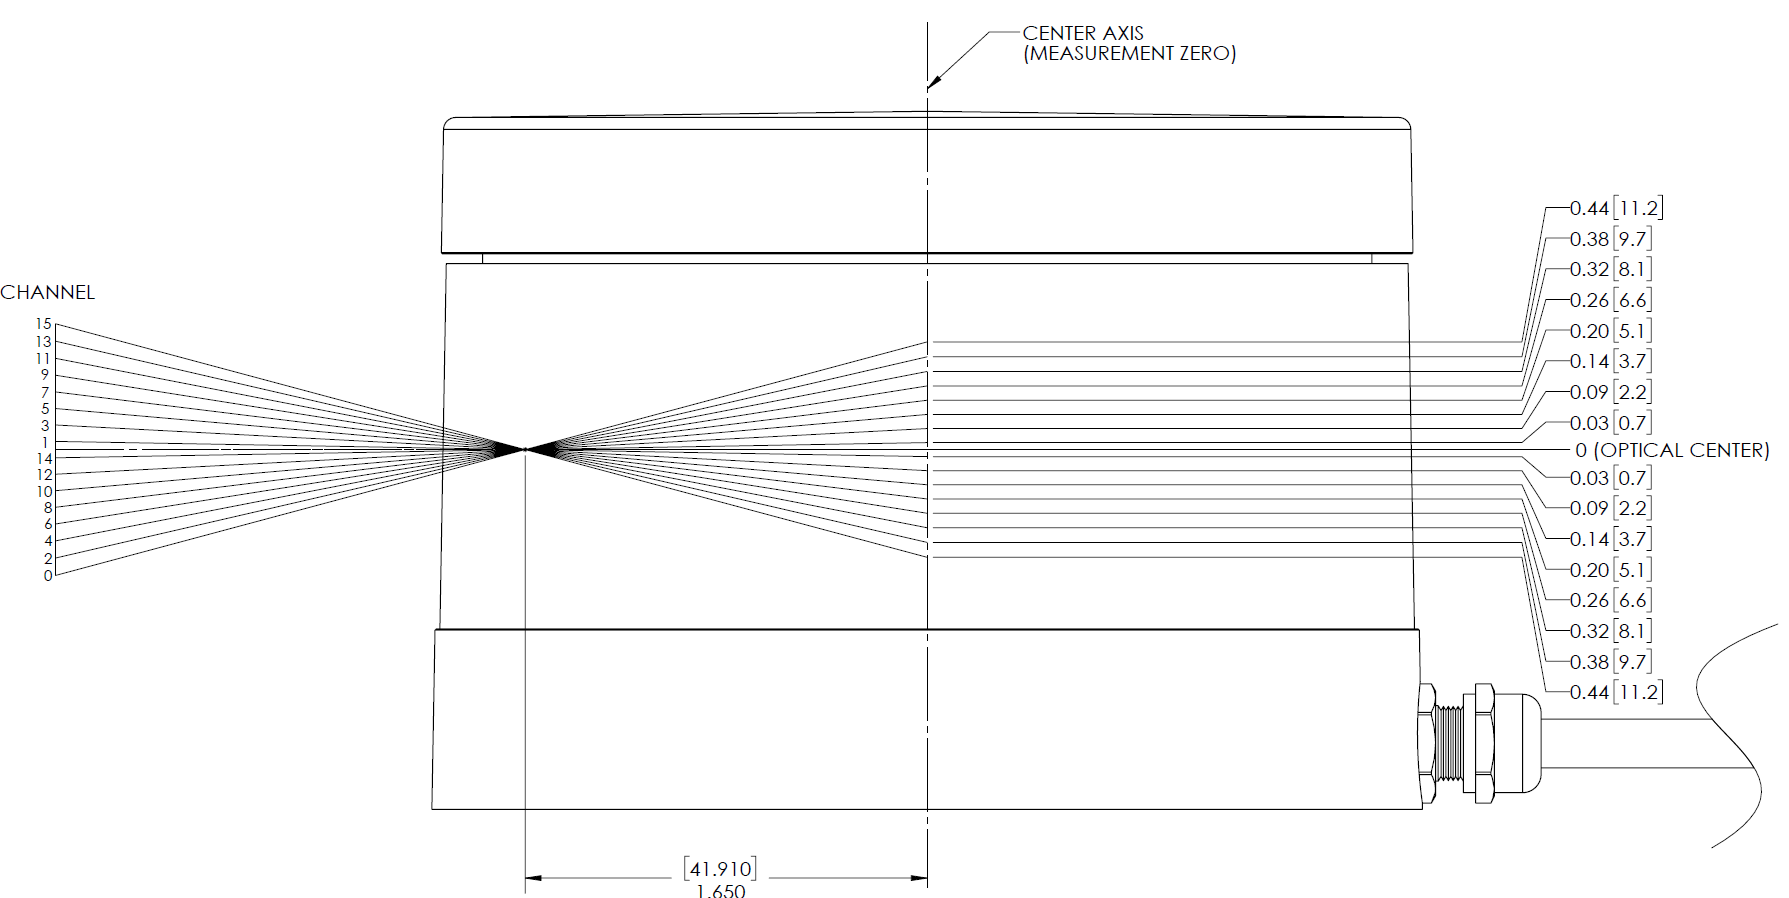
\includegraphics[width=0.8\textwidth]
	{resources/velodyne_channels.PNG}
	\caption[Laserstrahlen des Velodyne  VLP-16]{Laserstrahlen des Velodyne  VLP-16} \protect\cite{velodyne}
	\label{fig:angleVLP}
\end{figure}

Eine relevante Eigenschaft dieses Laserscanners ist die grosse Messdistanz, die Distanzen zwischen 0.3 m bis 100 m ermöglichen. Dabei ist die typische Toleranz +/- 3 cm. Der Reflektionsgrad wird in 256-bit Auflösung angegeben, d.h., dass der Sensor aus der zurückgesendeten Laserimpulsen die Intensität messen kann.

Der VLP-16 benötigt eine separate Interface Box, mit der die Speisung und die Datenschnittstellen zu einem 8-adrigen Kabel zusammengeführt werden. Die Adern 1-4 werden für die Ethernet Datenübertragung benötigt. Die Adern 5 und 6 sind nur bei zugeschaltetem \ac{GPS} nötig, ansonsten sind diese unbenutzt. Die stabilisierte 12 Volt Spannung wird über die Adern 7 und 8 zugeführt. Die Interface Box ist in Abbildung \ref{fig:InterfaceBox} ersichtlich. Diese besitzt folgende Anschlüsse; eine 12 Volt Speisung, einen Ethernet RJ45-Anschluss und eine \ac{GPS} Schnittstelle. Für die typische Leistungsaufnahme des Sensors wird 8 Watt angegeben. Aus einem Messaufbau konnte bei 12 Volt Speisespannung einen Strom von 0.6 Ampere ermittelt werden. Im Einschaltmoment kann der Strom kurzzeitig auf 0.9 Ampere ansteigen. Dies muss bei der Dimensionierung der Speisung beachtet werden.  

\begin{figure}[H]
	\centering
	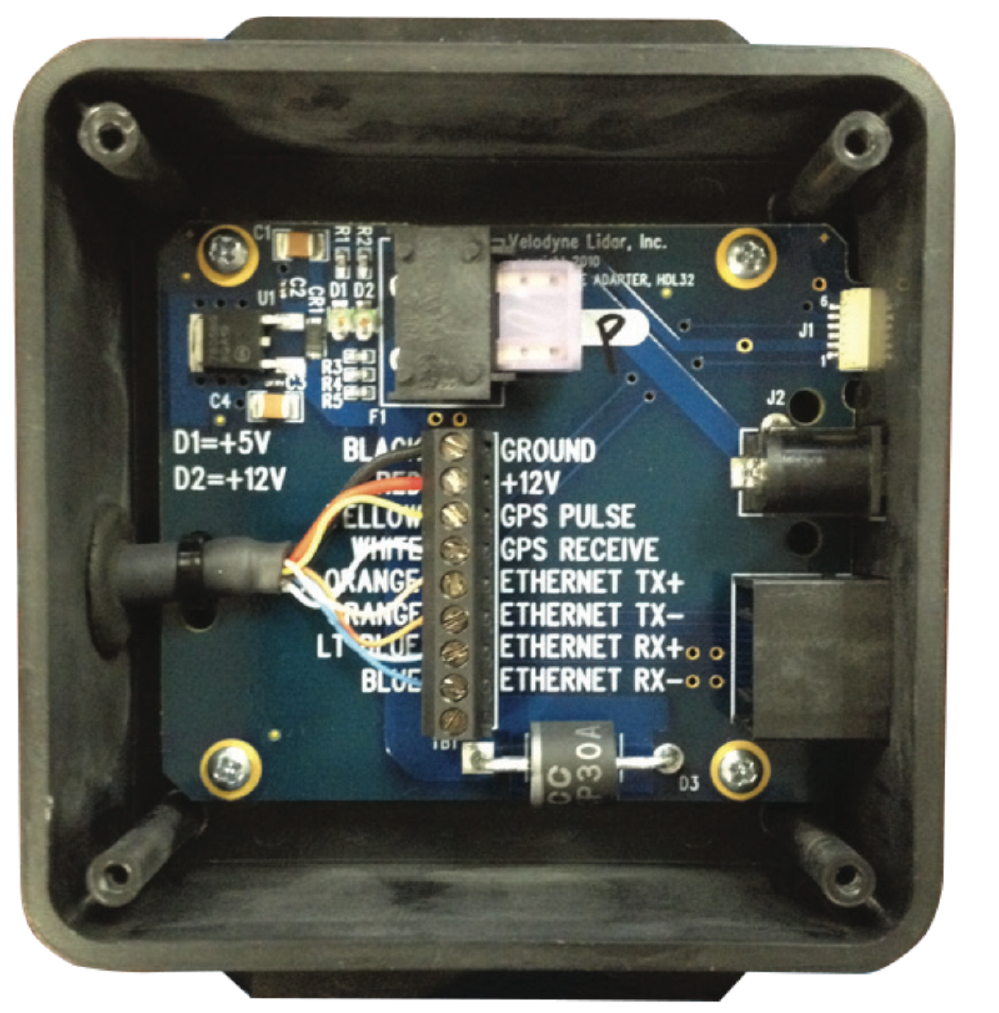
\includegraphics[width=0.5\textwidth]
	{resources/InterfaceBox.PNG}
	\caption[Ansicht auf die Interfacebox]{Ansicht auf die Interface Box} \protect\cite{velodyne}
	\label{fig:InterfaceBox}
\end{figure}

Über die Ethernetverbindung werden die Daten- und Positionspakete vom Velodyne an den Computer übermittelt. Dabei werden für die zwei verschiedenen \ac{UDP} Pakete die Ports 2368 und 8308 gebraucht. Nachfolgend wird in Abbildung \ref{fig:datapakets} der Aufbau eines Datenpakets dargestellt.

\begin{figure}[H]
	\centering
	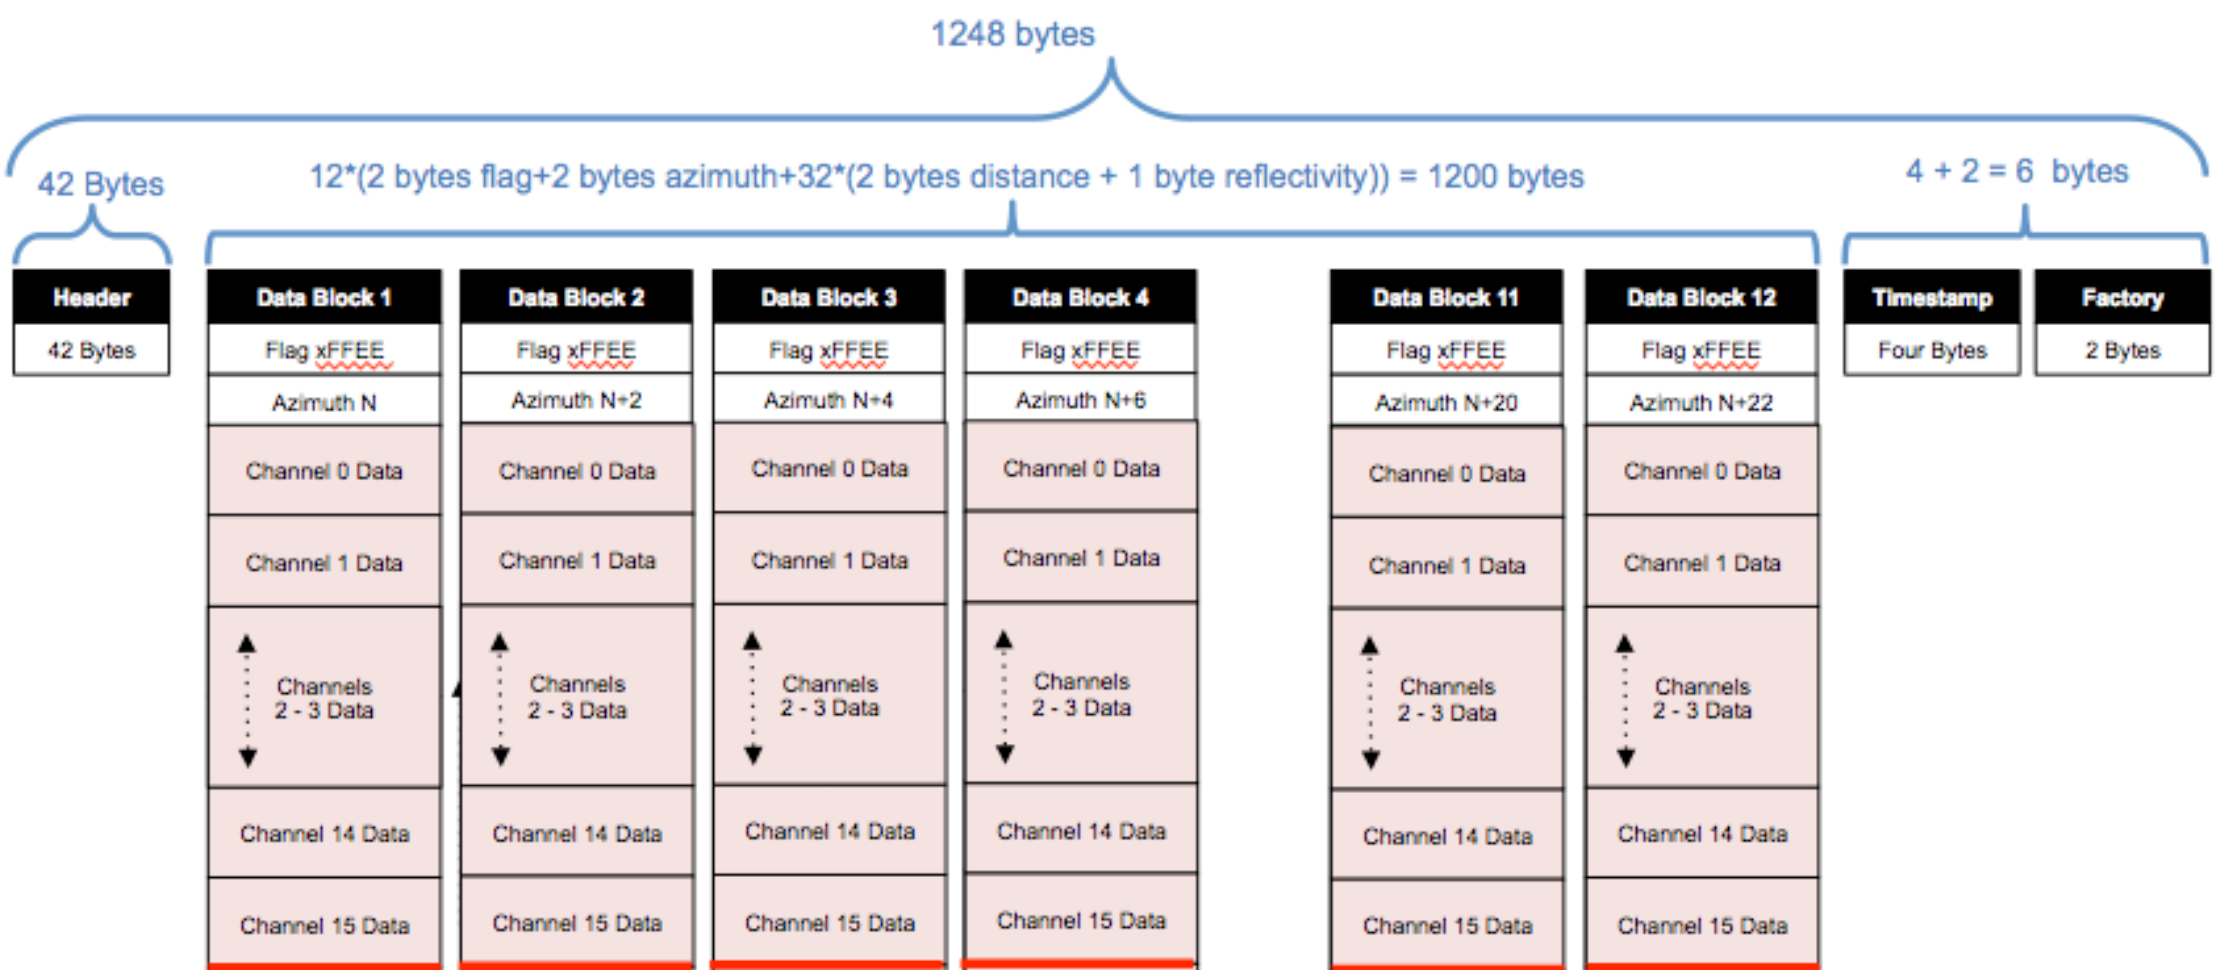
\includegraphics[width=1.0\textwidth]
	{resources/datapakets.PNG}
	\caption[Aufbau Datenpaket]{Aufbau Datenpaket} \protect\cite{velodyne}
	\label{fig:datapakets}
\end{figure}

 Jedes Paket besitzt einen 42-Byte Header und einen Datenblock, der aus Laserrückgabewert, kalibrierten Reflektionsgrad, Azimutwert und Zeitstempel besteht. Ein einzelnes Datenpaket besitzt die Grösse von 1248 Bytes und beinhaltet die Datensätze aller 16 Laserkanäle. Die typische Datenübertragungsrate wird mit 8 Mbit/s angegeben.

\section{Stand der Technik}
 \label{sec:Vorzeigeprojekte}
 Dieses Kapitel dient als Vorstudie über den Einsatz des Velodyne VLP-16 durch bereits bestehende Projekte. Dabei werden zwei verschiedene Konfigurationen betrachtet und dazu entsprechend Vor- und Nachteile erläutert. Es handelt sich hierbei um zwei Teams, welche an der \ac{EnRicH} 2017 teilgenommen haben und als State-of-the-Art Projekte betrachtet werden.
 
 \subsection{IMM MSAS Team MSS Warschau}
 \label{subsec:IMM}
Das Institute of Mathematical Machines (IMM) in Warschau hat den Velodyne VLP-16 an einer endlos drehenden Konstruktion befestigt. Dabei ist der Sensor nicht in der üblichen Lage (Ausrichtung XY-Ebene), sondern um 90$^\circ$ abgedreht (Ausrichtung YZ Ebene). In Abbildung \ref{fig:imm} ist die entsprechende Konfiguration abgebildet. 

   \begin{figure}[H]
	\centering
	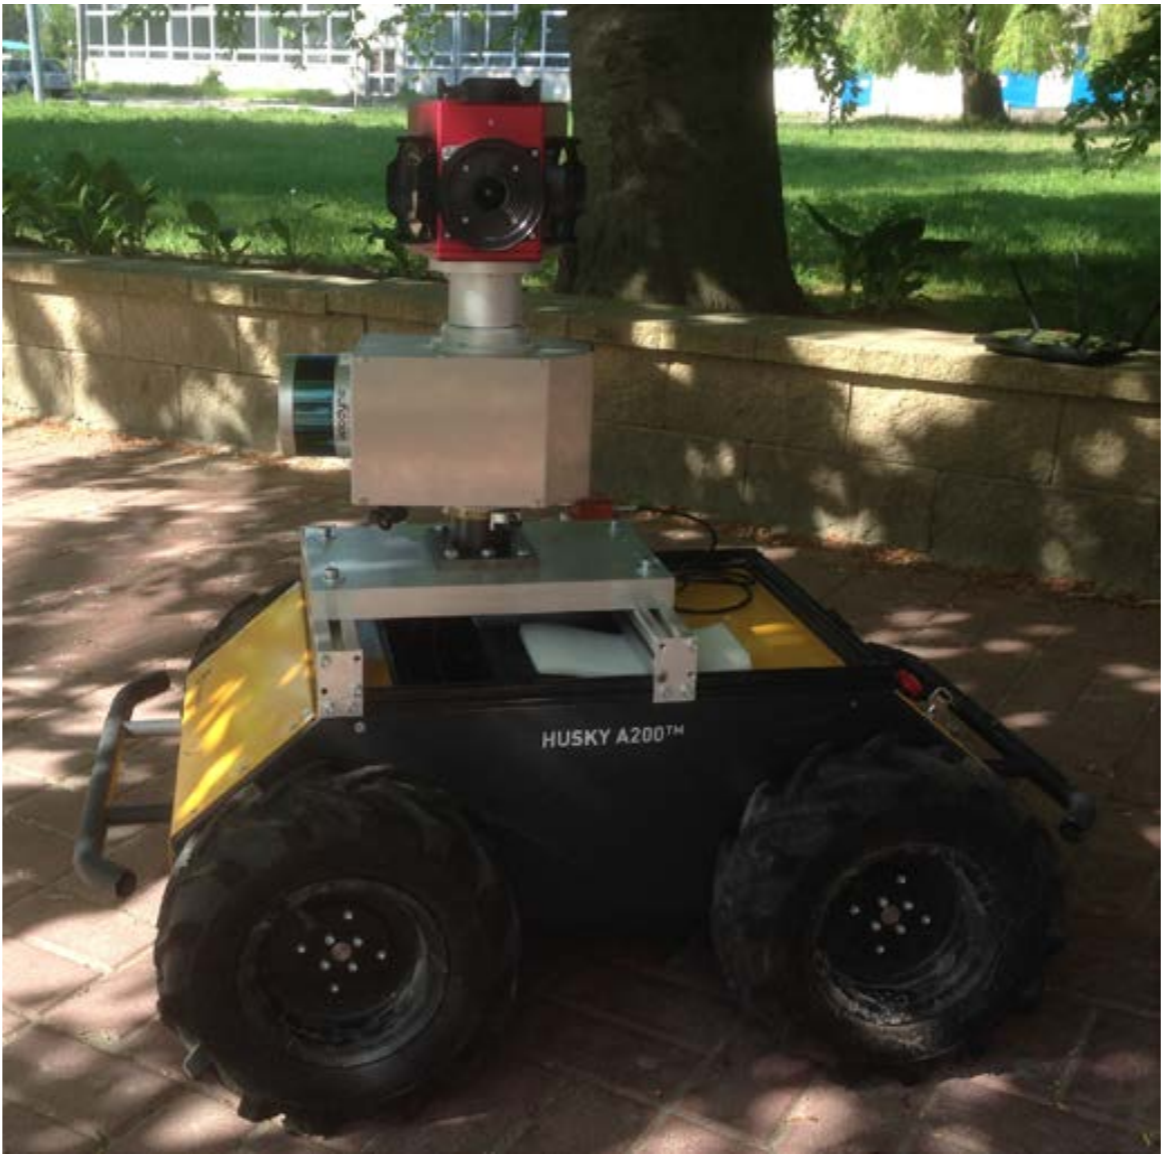
\includegraphics[width=0.7\textwidth]
	{resources/IMM.PNG}
	\caption[Roboter des Team IMM EnRicH]{Roboter des Team IMM an der EnRicH} \protect\cite{IMM}
	\label{fig:imm}
\end{figure}

In der nachfolgenden Betrachtung wird vom Koordinatensystem der Abbildung \ref{fig:imm} ausgegangen.
Das Team nutzt bei dieser Konfiguration die begrenzte Auflösung des Sensors besser aus. Die vertikale und horizontale Auflösung wechseln dabei. Ist die Konstruktion nicht drehend, kann er in der Vertikalen den Bereich 360$^\circ$ mit der Auflösung von 0.01$^\circ$ - 0.04$^\circ$ messen. In der Horizontalen kann der Bereich 30$^\circ$ mit 2$^\circ$ aufgelöst werden. 

Der Vorteil dieser Konfiguration wird jedoch erst durch die Rotation um die Z-Achse deutlich. Wird der Sensor nun kontinuierlich um die Z-Achse gedreht, verschieben sich die 16 horizontalen Laserstrahlen mit der Umdrehungsgeschwindigkeit der Konstruktion. Einerseits bewegt sich der 30$^\circ$ grosse Messkegel durch den Raum und kann somit 360$^\circ$ in der Horizontalen vermessen. Anderseits kann durch die interne Rotation des Sensors 360$^\circ$  in der Vertikalen ausgemessen werden. Die schlechtere Auflösung von 2$^\circ$ kann somit kompensiert werden, da sich die Laserstrahlen kontinuerlich verschieben. Diese Konfiguration ermöglicht eine detaillierte Messung, da jeder Punkt im Raum von 16 Laserstrahlen mit der Auflösung zwischen 0.1$^\circ$ - 0.4$^\circ$ durchlaufen wird. 

Die oben erläuterte Betrachtung gilt jedoch nur, wenn die Umdrehungsgeschwindigkeit der Konstruktion bedeutend langsamer als die interne Umdrehungsgeschwindigkeit des Sensor ist. Ansonsten besteht die Gefahr, dass die Reflektion des Laserstrahls nicht detektiert werden kann. Die Auflösung ist direkt von der Umdrehungsgeschwindigkeit der Konstruktion abhängig. Es wird zusätzlich davon ausgegangen, dass keine zusätzliche Translation, d.h. Bewegung des Roboters, stattfindet. Diese Konfiguration eignet sich somit, wenn das zu vermessende Gelände bekannt ist. Dadurch können vordefinierte Positionen angesteuert werden, an denen eine halbe Umdrehung ausreicht, um eine räumliche Messung an der definierten Position zu erstellen. 

Weiter wird in der obigen Betrachtung die Abweichung zur Drehachse komplett vernachlässigt. Es entsteht ein Messfehler, der dem Abstand des Sensors zur Drehachse entspricht. Ein weiterer Messfehler kann durch Translation entstehen, wenn sich das Fahrzeug bewegt. Diese zwei Messfehler lassen sich jedoch durch Koordinatentransformationen in ein festes Koordinatensystem verschieben. Die Schwierigkeit dabei ist, die exakten Messewerte mittels einem Drehencoder und einer \ac{IMU} zum jeweiligen Zeitpunkt zu ermitteln. 

Ein Nachteil für die Aufgabenstellung ist, dass bei dieser Konfiguration im freien Feld viele Messpunkte ins Leere messen, da himmelwärts (Richtung Z-Achse) keine Objekte als Reflektor dienen. Auch Messpunkte in Richtung negative Z-Achse müssen gefiltert werden, da ansonsten ständig die Oberfläche des Roboter selbst reflektiert wird.

\subsection{Hector Tracker Team Hector Darmstadt}
 \label{subsec:hector}
Das Team Hector der Universität Darmstadt besitzt auf dem Hector Tracker eine weitere Konfigurationsmöglichkeit. Auch dieses Team arbeitet mit einem endlos drehenden Konstruktion. Bei nachfolgenden Betrachtungen wird vom Koordinatensystem in Abbildung \ref{fig:hector} ausgegangen. Der Velodyne VLP-16 befindet sich 45$^\circ$ abgeneigt zur XZ-Ebene. Dabei ist die Lage des Sensors zentral auf der Drehachse Z.

\begin{figure}[H]
	\centering
	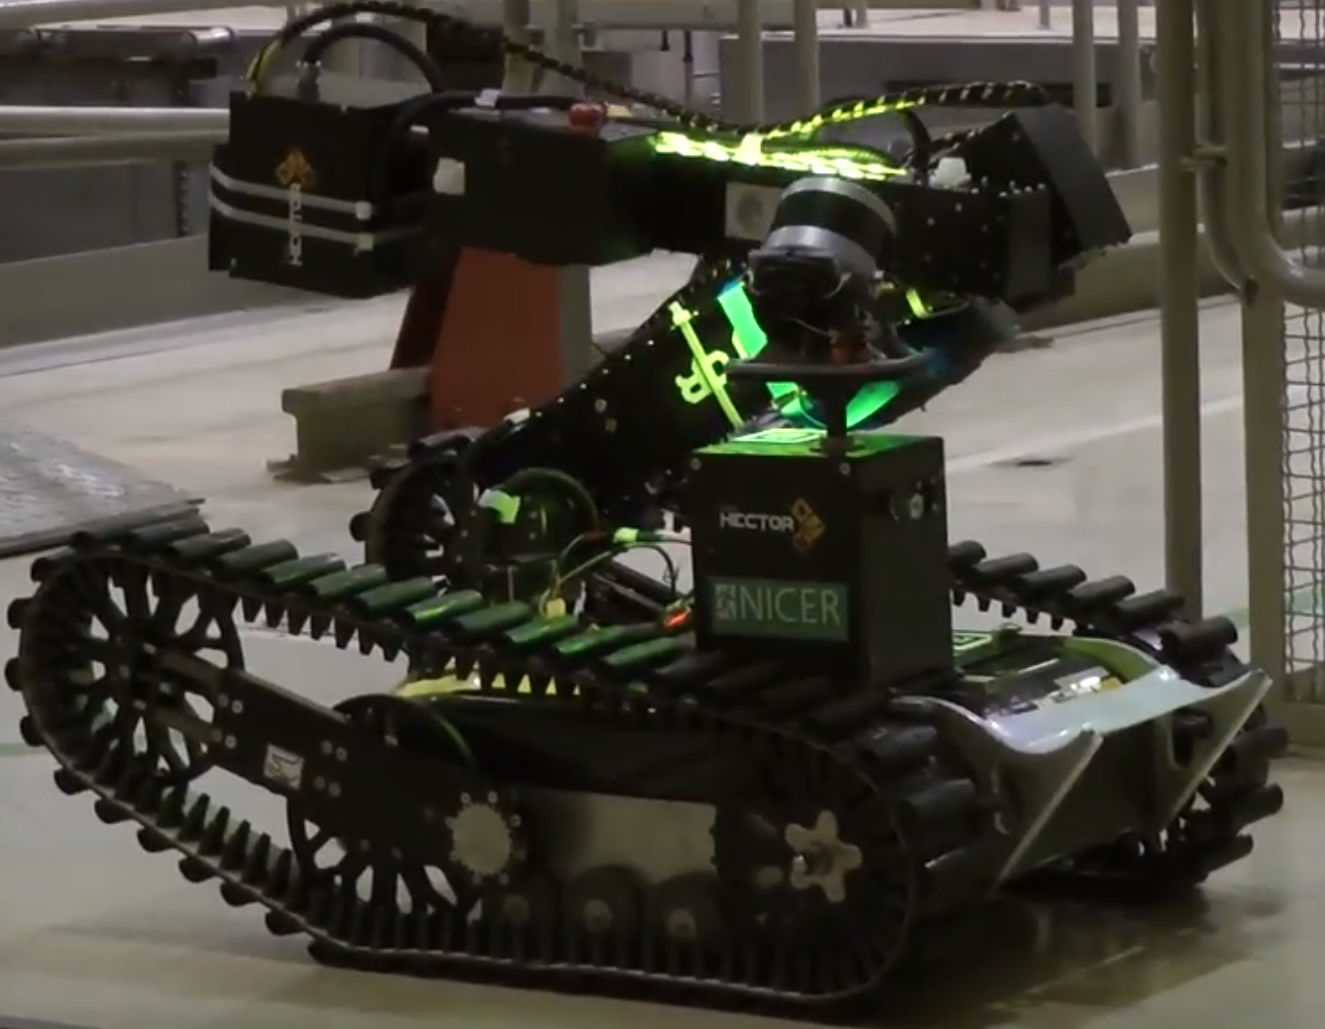
\includegraphics[width=0.7\textwidth]
	{resources/hector.PNG}
	\caption[Roboter des Team Hector EnRicH]{Roboter des Team Hector an der EnRicH} \protect\cite{hector}
	\label{fig:hector}
\end{figure}

Im stationären Zustand kann durch diese Konfiguration keine Verbesserung der Auflösung erreicht werden. Die Auflösungen bleiben erhalten, sind jedoch nun entsprechend der Neigung um 45$^\circ$ verschoben. Durch die Neigung des Sensors wird der Raum nicht gleichmäßig vermessen. 

Die räumliche Vermessung wird auch hier erst mit der Rotation um die Z-Achse ermöglicht. Gegenüber einer festen nicht drehenden Lösung besitzt diese Konfiguration somit den Vorteil, dass Messpunkte, welche sich zwischen den Laserstrahlen befinden, durch Drehen erreichen lassen. Dabei wird der 30$^\circ$ Messkegel durch die Rotation ständig im vertikalen Bereich hin- und hergeschoben.

Es kann während einer Umdrehung somit durch die Neigung von 45$^\circ$ und dem 30$^\circ$ Kegel des Sensors eine Abdeckung in der Vertikalen von 240$^\circ$ erreicht werden. Die horizontale Abdeckung bleibt hierbei weiterhin 360$^\circ$, da der Sensor die interne Rotation vollführt.

Auch bei dieser Betrachtung  muss die Umdrehungsgeschwindigkeit der Konstruktion bedeutend langsamer als die interne Umdrehungsgeschwindigkeit des Sensor sein. Die Auflösung bei dieser Konstruktion ist direkt zur Umdrehungsgeschwindigkeit abhängig. Des Weiteren muss bei dieser Konfiguration die Translation, d.h. die Bewegung des Roboters, noch separat korrigiert werden.  

Im Vergleich zum Projekt der IMM entstehen bei dieser Konfiguration weniger Messpunkte in Richtung des Roboters und in Richtung der Z-Achse (himmelwärts). Dies ist für Raum interne Messungen unvorteilhaft. Für die Messung im freien Feld ist diese Konfiguration besser geeignet, sofern sich keine hohe Objekte in unmittelbarer Nähe des Sensor befinden. 
 	
\subsection{Schlussfolgerung}
An der \ac{EnRicH} 2017 nutzen mehrere Teams den Velodyne VLP-16 mit unterschiedlichen Konfigurationen. Die zwei betrachteten Konfigurationen nutzen die Möglichkeit einer endlos drehenden mechanischen Konstruktion. Im Unterkapitel \ref{sec:Antriebsmoeglichkeiten} werden mögliche Antriebsmöglichkeiten für eine solche Konstruktion evaluiert. Eine endlos drehende Konstruktion benötigt ein spezielles Handling der Kabelführung, daher wird im Unterkapitel \ref{subsec:Schleifring} die Möglichkeit eines Schleifrings beschrieben. Beide Konfiguration besitzen Vor- und Nachteile bei der Umgebungserkennung. Um eine möglichst detaillierte Umgebungswolke zu erstellen müssen vorwiegend Translation und Rotation um die Drehachse kompensiert werden. Diese lassen sich durch Koordinatentransformation und entsprechender Sensorik ermöglichen. In Unterkapitel \ref{sec:position} werden dazu mögliche Varianten zur Positionsbestimmung erläutert.
  
\section{Software}
\label{sec:Software}
In diesem Kapitel wird die notwendige Software beschrieben. Es erläutert das \ac{ROS} und dessen Funktion im Projekt. Daneben werden weitere Softwareapplikationen und -packages erwähnt, welche für die Aufgabenstellung nützlich sind.

\subsection{ROS Robot Operating System}
\label{subsec:ROS}
Die gesamte Kommunikation mit Sensoren und Aktoren findet auf dem Packbot mit \ac{ROS} statt. Da das 3D-Laser-Modul auf dem Packbot, aber auch selbstständig funktionieren soll, ist ROS nicht zwingend einsetzbar. Dennoch wurde für die Aufgabenstellung ROS gewählt. Im Zusammenhang mit Velodyne und 3D-Mapping bietet ROS neben Visualisierungtools und bereits bestehender Treiber-Packages auch die Integrationen der \ac{PCL}. Die \ac{PCL} ist eine umfangreiche Softwarebibliothek, welche viele Funktionen und Codebeispiele bereit stellt, um Punktwolken zu erstellen.

Grundsätzlich wird \ac{ROS}, wegen seiner Nähe zu Linux Distributionen, auf einem Ubuntu Betriebssystem aufgesetzt und ist ein Software-Framework, dass die Programmiersprachen C++ und Python nutzt. Diese in 2007 entwickelte Open Source Software erhielt in den letzten Jahren ständig neue und überarbeitete Versionen.

Die Empfehlung von ROS und diversen Literaturen liegt bei der neusten Distribution ROS "Kinetic Kame". \cite{ROSprojects} Es handelt sich um eine Langzeitversion, welche bis 2021 Unterstützung bietet. Im Zug der ersten Versuchen mit ROS wurde auf einem Laptop mit \ac{AMD64}-Architektur gearbeitet. Auf diesem wurde ROS Kinetic Kame voll umfänglich ermöglicht. Damit das 3D-Lasermodul selbständig agieren kann, wird jedoch ein einbaubarer Einplatinencomputer benötigt. In Unterkapitel \ref{sec:Datenverarbeitung} werden aktuelle Einplatinencomputer beschrieben. 

Während der Einarbeitung mit Kinetik Kame konnten einige Nachteile der Distribution festgestellt werden. Es wurde festgestellt, dass diverse Packages nur für \ac{AMD64}-Architekturen zur Verfügung stehen und nicht für \ac{ARM}-Architekturen \cite{armhf_issues}. Dies könnte zu Eingrenzungen während der Realisierung führen, daher werden nötige Packages geprüft.
\newpage
\subsection{Velodyne Package}
Wie bereits im vorherigen Kapitel erwähnt, besitzt ROS ein Treiber-Package für den Velodyne VLP-16. Dieses Package wird für ARM- und AMD64-Architekturen ermöglicht. In der Abbildung \ref{fig:rosgraph} ist der Aufbau dieses Treibers mit dem ROS-Tool rqt-graph visualisiert. 

\begin{figure}[H]
	\centering
	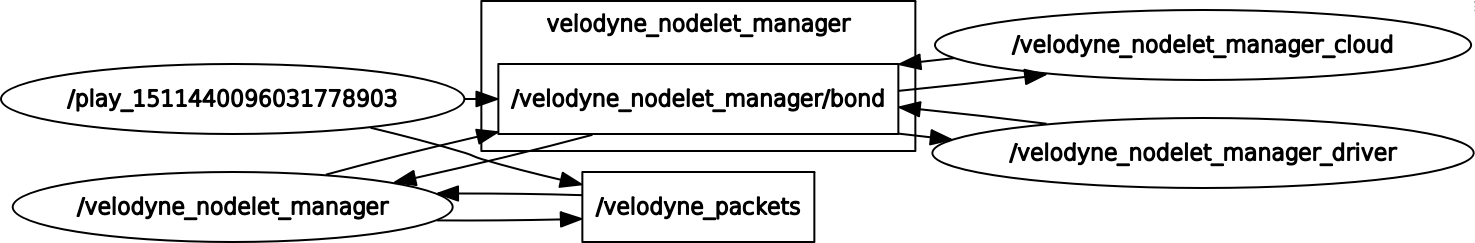
\includegraphics[width=1\textwidth]{resources/rosgraph.png}
	\caption[Velodyne Treiber aus rqt-graph ]{Velodyne Treiber aus rqt-graph}
	\label{fig:rosgraph}
\end{figure} 

Dieses Package vereinfacht die Sensordatenverarbeitung bedeutend. Mittels dem Package werden die hexadezimalen Rohdaten von den Ethernet-Datenpaketen aus Abbildung \ref{fig:datapakets} bereits ausgewertet und kalibriert zur Verfügung gestellt. Dabei laufen mehrere Programmsegmente (\textit{Nodes}) parallel. 

Für die Aufgabenstellung ist nur der Node velodyne\_packets relevant, da dieser den verarbeiteten Sensor-Datenstream zur Verfügung stellt. Es werden dabei zwei unterschiedliche Typen von \textit{Messages} kontinuerlich ausgegeben \textit{(published)}. Die Message \textit{velodyne\_packets (vom Typ: velodyne\_ msgs/VelodyneScan)} beinhaltet die Rohdaten eines einzelnen Laserstrahls. Die Message \textit{velodyne\_points (vom Typ: sensor\_msgs/PointCloud2)} beinhaltet die angesammelten Datenpunkte, welche bereits zu einem festen Koordinatensystem fixiert sind \cite{ROSvelodyne}.

Das Package bietet die Abstraktion der Datenerfassung und Integration in ein festes Koordinatensystem. Werden die PointCloud2 Messages zusammengefügt und mittels Koordinatentransformation räumlich angepasst, lässt sich somit eine Umgebungsabbildung erzeugen.
\begin{figure}[H]
	\centering
	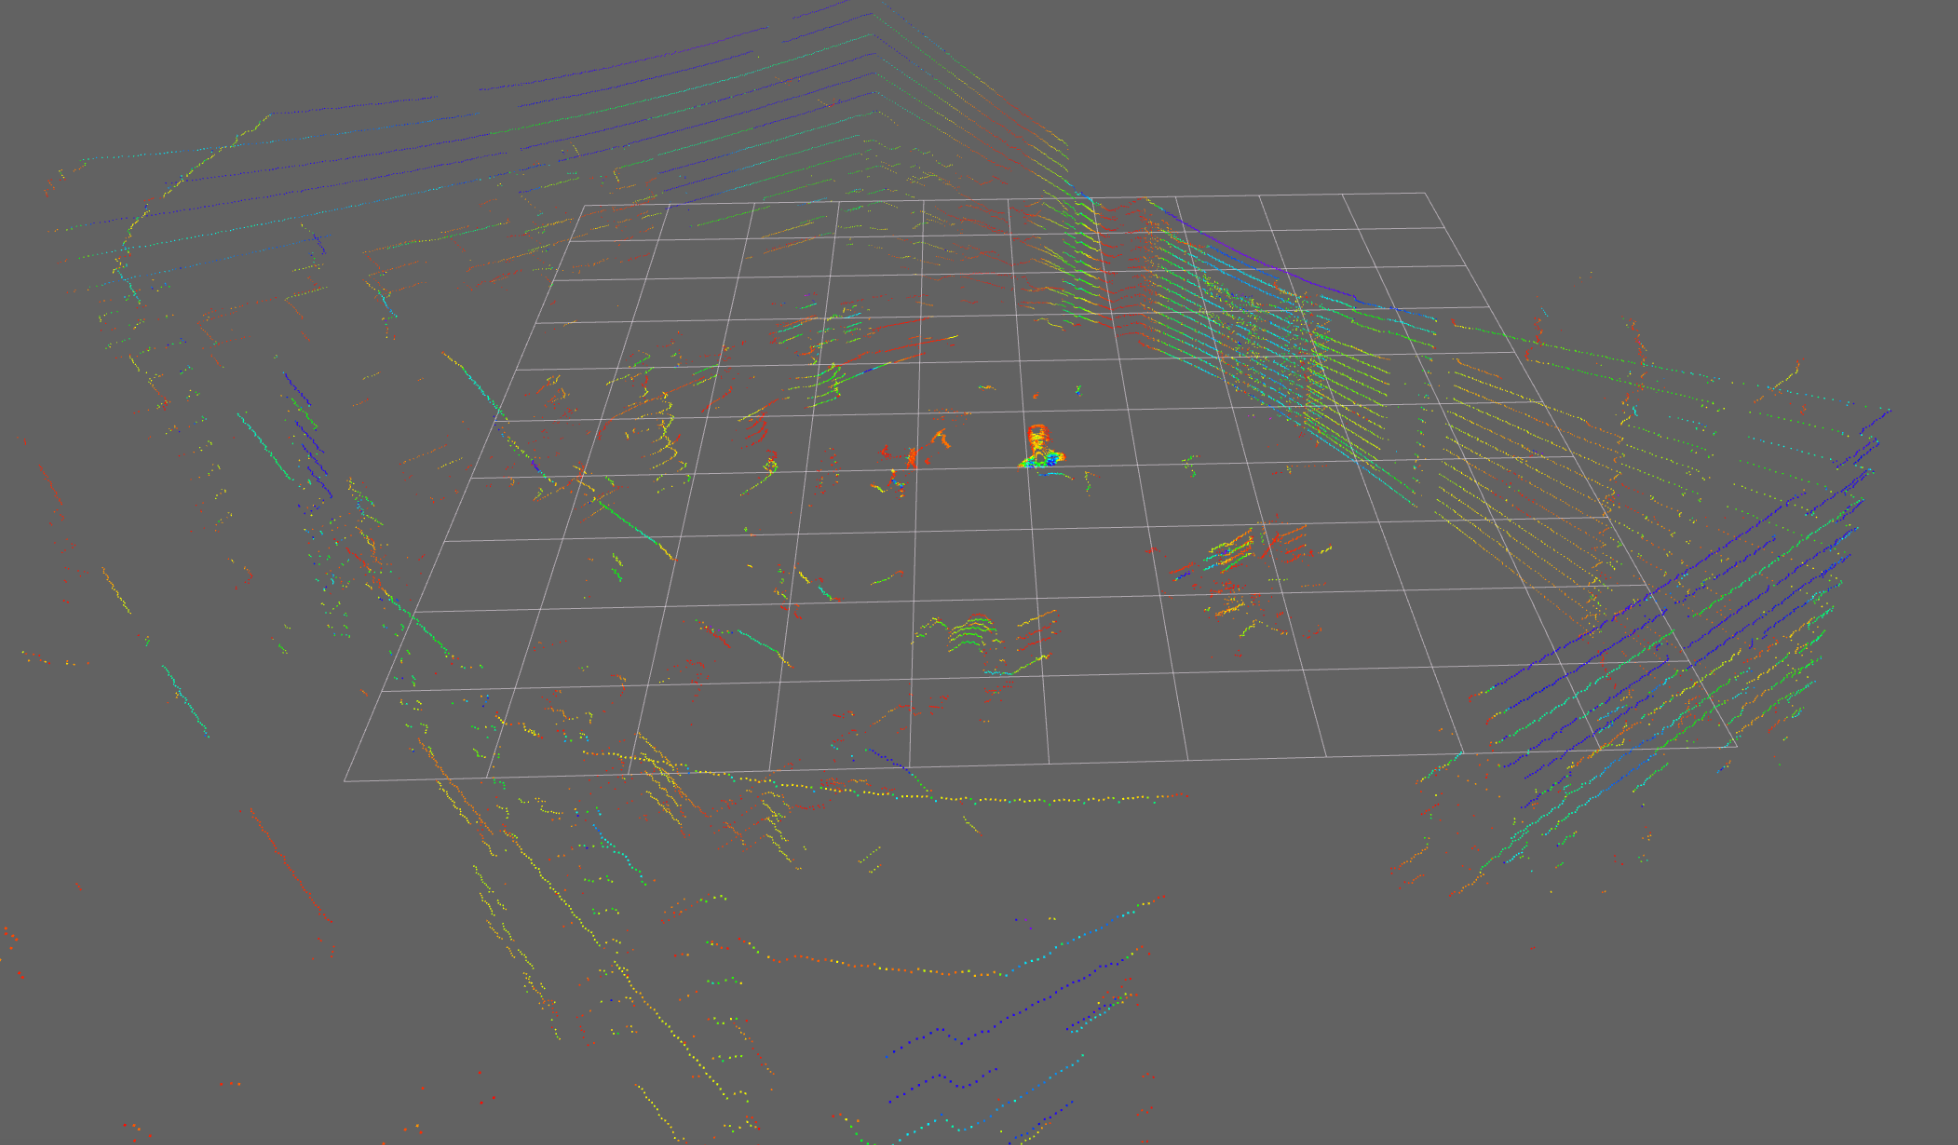
\includegraphics[width=0.8\textwidth]{resources/rviz.PNG}
	\caption[PointCloud2 Datenstream mit Rviz]{PointCloud2 Datenstream mit Rviz}
	\label{fig:rviz}
\end{figure} 

Mittels dem ROS-Tool Rviz lässt sich der Datenstream über velodyne\_packets direkt visualisieren. In Abbildung \ref{fig:rviz} ist ein statischer Datenstream visualisiert. Dies geschieht, indem das Tool kontinuierlich die Messages empfängt \textit{(subscribed)}.

ROS bietet zudem die Möglichkeit über den \textit{rosbag}-Befehl Messungen aufzunehmen und abzuspeichern. Dies ermöglicht somit nicht nur den aktuellen Sensordatenstream zu visualisieren, sondern auch getätigte Messungen zu archivieren \cite{ROSTutorials}. 

\subsection{Schlussfolgerung}
Für die Aufgabenstellung eignet sich ROS gut, wegen den bereitstehenden Tools und den Packages, mit denen ein grosser Teil der Software abstrahiert werden kann. Der aktuelle Code muss um einige Nodes erweitert werden. Die einzelnen Sensordaten werden einerseits auf die aktuelle Position verschoben und anderseits zu einer einzigen Punktwolke zusammengefügt. Die Einarbeitung mit ROS ist jedoch relativ umfangreich und bietet eine Vielzahl an Tools und eine Softwarearchitektur, die zuerst kennen gelernt werden müssen.  

\section{Datenverarbeitung}
\label{sec:Datenverarbeitung}
Um die Datenmenge zu verarbeiten und die Ansteuerung der Komponenten zu realisieren, eignen sich Einplatinencomputer. Einplatinencomputer besitzen den Vorteil, dass sie gegenüber üblichen Mikroprozessoren grössere Speichermöglichkeiten, höhere Prozessorleistungen und bootbare Betriebssysteme ermöglichen. Gegenüber \ac{XPC} besitzen sie den Vorteil, dass sie Hardware näher sind, indem sie direkt ansteuerbare Pins besitzen (GPIOs). Aus diesem Grund werden nachfolgend diverse Einplatinencomputer betrachtet. Kriterien bei der Auswahl eines geeigneten Boards sind Prozessorleistung, \ac{RAM}, Preis, Ethernet-Schnittstelle, Speichermöglichkeit, GPIO-Verfügbarkeit und die verbaubare Dimension. Diese Kriterien wurden durch die Vorgaben des Pflichtenhefts im Anhang \ref{Anhang} festgelegt. Geeignete Prozessorleistung, Speichermöglichkeit und \ac{RAM} sind für die erfolgreiche Verarbeitung der Sensordaten nötig, da die Punktwolke mit zunehmender Zeit an Datengröße zunimmt. Die Datenübermittlung des Velodyne und des Packbots erfolgt über Ethernet, daher benötigt der Einplatinencomputer mindestens einen RJ45-Anschluss.

\subsection{Raspberry Pi 2 \& 3}
\label{subsec:Raspberry}
Das Raspberry Pi ist eines der bekanntesten Einplatinencomputer und bietet daher eine grosse Community. Da bereits ein Raspberry Pi 2 zur Verfügung gestanden ist, konnten die ersten Erfahrungen mit einem Raspberry Pi gemacht werden. Das Raspberry bietet zusammen mit ROS Kinetic Kame und Ubuntu Mate LTS 16.04 eine Lösung für die Datenverarbeitung. Das Raspberry Pi 2 bzw. 3 basiert auf einem Broadcom \ac{SOC} und ist mit einem \ac{ARM} Cortex A7 bzw. A53 Prozessor mit vier Kernen ausgestattet. Die Taktfrequenz liegt bei diesem lediglich bei 1.2 GHz. Beide Modelle besitzen 1 GB \ac{RAM}. Das Betriebssystem wird auf einer \ac{SD} gebootet. Speichermöglichkeiten sind über USB oder die SD-Karte vorhanden. Auch GPIOs und eine Ethernetschnittstelle sind beim Raspberry Pi vorhanden. Der Preis eines Raspberry Pi liegt momentan bei ca 50 Fr. \cite{rpi}

\subsection{Banana Pi M3}
\label{subsec:BananaPi}
Der Banana Pi M3 bietet zur Zeit (Stand Oktober 2017) die höchste Performance bei Einplatinencomputern mit \ac{ARM}-Architektur durch den Allwinner A83T Achtkern-Prozessor, der mit 1.8 GHz taktet und den 2 GB RAM. Neben USB-Anschlüssen bietet es eine SATA-USB-Schnittstelle, die den internen 8 GB \ac{eMMC}-Speicher um bis zu 2 TB erweitern lässt. Es bietet auch direkt integrierte WLAN-Schnittstellen, sowie eine RJ45 Gigabit Netzwerkschnittstelle. Der Preis eines Banana Pi M3 liegt momentan bei ca 90 Fr.. Im Zusammenhang mit Banana Pi M3 und Ubuntu werden mehrfach Komplikationen und Probleme veröffentlicht \cite{rpi} \cite{banana}. Dies ist ein bedeutender Nachteil für dieses Einplatinencomputer. 

\subsection{Odroid C2 \& XU4} 
\label{subsec:Odroid}
In diversen Literaturen (siehe \cite{ROSprojects} Kapitel 4) werden neben dem Raspberry Pi, Odroid Boards als empfohlene Einplatinencomputer aufgelistet. Dabei stehen die aktuelle Modelle Odroid-C2 oder Odroid-XU4 zur Verfügung. Sie bieten eine höhere Prozessorleistung, 1.5 GHz bzw. 2 GHz mit je 2 Gigabyte \ac{RAM}. Betriebssysteme können via \ac{SD} oder \ac{eMMC} gebootet werden. Beide Boards sind jedoch noch nicht lange auf dem Markt und bieten in vielen Anwendungen nur Beta-Versionen. Vor allem die Unterstützung von Ubuntu LTS 16.04 ist nicht restlos geklärt. \cite{ubuntuodroid} Der Preis dieser Boards liegt bei ca. 80 - 90 Fr. \cite{rpi}.

\subsection{Up Board Squared} 
\label{subsec:Up Board Squared}
Dieser Einplatinencomputer unterscheidet sich wesentlich von den bisherig betrachteten Boards. Der Prozessor arbeitet nicht mit \ac{ARM}-Architektur, sondern mit \ac{AMD64}-Architektur. Somit können Ubuntu und ROS Distributionen voll umfänglich genutzt werden. Er besitzt mit Intel Pentium ein vier kerniger Prozessor und taktet mit 2.5 GHz. Zusätzlich bietet er einen separaten 500 MHz \ac{GPU} und bis zu 8 GB \ac{RAM}. Neben USB werden auch zwei RJ45-Schnittstelle und ein GPIO Pinlayout angeboten, welches dem des Raspberry Pis entspricht. Das Up Board Squared bietet sich an, falls die Performance und die Kompatibilität der ARM-Architektur mit ROS nicht ausreicht. Der Preis eines Up Board Squared kostet je nach Ausführung zwischen 180 - 380 Fr..

\subsection{Schlussfolgerung}
\label{subsec:Schlussfolgerung}
Für die Aufgabenstellung eignet sich lediglich das Raspberry Pi 2 oder 3, um ROS mit Ubuntu LTS 16.04 zu betreiben. Das Banana Pi und die Odroid Boards sind im Kriterium Speichermöglichkeit und Prozessorleistung besser geeignet, können jedoch wegen fehlender Betriebssystem-Kompatibilität nicht genutzt werden. Die Dimensionen aller betrachteten Boards sind, mit Ausnahme des Up Board Squared sehr kompakt. Im Punkt Ethernetschnittstelle bietet lediglich das Up Board Squared zwei Ethernetanschlüsse, mit welchen ein zusätzlicher Ethernet Switch hinfällig wird. Das Up Board Squared bieten in fast allen Kriterien eine bessere Lösung. Aus Kostengründen wurde für den zu erarbeitenden Prototypen das Raspberry Pi als genügend bewertet. Für eine allfällige Optimierung bietet sich das Up Board Squared an.

\section{Antriebsmöglichkeiten}
\label{sec:Antriebsmoeglichkeiten}
Um den Velodyne VLP-16 um eine Achse drehen zu lassen, müssen Motoren eingesetzt werden. Nachfolgend werden zwei verschiedene Motorenarten beschrieben, welche sich für die Aufgabenstellung eignen. Wichtige Kriterien für die Aufgabenstellung sind die Ansteuerung und die Dimension. Zudem muss die Möglichkeit bestehen die Winkeländerung zu eruieren. 

\subsection{Schrittmotor}
\label{subsec:Schrittmotor}
Der Schrittmotor ist eine Antriebsmöglichkeit, welche für das Projekt in Frage kommt. Es gibt sehr kostengünstige und kompakt dimensionierte Motoren dieser Art. Ein interessanter Aspekt ist das gezielte Steuern des Motors. Durch einen Stromimpuls bewegt sich ein Schrittmotor nur einen festgelegten Winkelschritt weiter. Er kann bereits ohne zusätzliche Sensorik definierte Schritte anfahren, aus denen die Winkeländerung eruiert werden kann. Schrittmotoren besitzen die Eigenschaft, dass in der Ruhelage ein Haltemoment entsteht. Diese Eigenschaft wird jedoch für die Aufgabenstellung nicht zwingend benötigt. Preislich muss bei einem geeigneten Schrittmotor mit 40 Fr. gerechnet werden. \cite{Trinamic} 

Nachteilig für die Aufgabenstellung am Schrittmotor ist der höhere Stromverbrauch, vor allem zum Aufbringen des Haltemoments. Da nur ein Schritt ausgeführt wird, wenn das entsprechende Drehmoment nicht überschritten wird, müsste dieses sorgfältig berechnet werden. Ein bedeutender Nachteil im Zusammenhang mit der Aufgabenstellung ist, dass durch Schrittverluste die Winkeländerung nicht mehr quantitativ ermittelt werden kann. Schrittmotoren mit integrierten Encodern würden in diesem Fall Abhilfe schaffen. Aus Kostengründen (Preise ab 300 Fr. \cite{mouserstepper}) wurden Schrittmotoren mit integrierten Absolutencodern nicht weiter vertieft. 
Ein weiterer Nachteil ist das verhältnismäßig hohe Gewicht. Dies ist kein Kriterium für die Aufgabenstellung, sollte jedoch bei der Realisierung beachtet werden.

Um mit einem Einplatinencomputer einen Schrittmotor anzusteuern, empfiehlt sich ein Schrittmotorentreiber. Mit solchen Treibern lässt sich der Motor mittels 2 Steuerpins rotieren. Um die Drehgeschwindigkeit zu senken, bieten diese Treiber die Möglichkeit, die Schritte in 2, 4, 8 und 16 Teilschritte zu senken. Es ermöglicht zudem eine feinere Bewegung. \cite{DRV8825}.

\subsection{Gleichstrommotor}
\label{subsec:Gleichstrommotor}
Als Alternative zum Schrittmotor bietet sich ein üblicher Gleichstrommotor. Diese Motoren sind für viele Einsatzbereiche geeignet und es gibt sie in verschiedenen Grössen und Umdrehungszahlen. Im Gegensatz zu Schrittmotoren laufen Gleichstrommotoren kontinuierlich, aufgrund eines Stroms, der durch die Wicklungen fliesst. Nachteilig ist somit, dass weder die genaue Anzahl der Umdrehungen noch die momentane Phasenlage bekannt ist. Es gibt jedoch eine Vielzahl an Möglichkeiten, diese zu eruieren. Einerseits gibt es die Möglichkeit mittels Hall-Sensoren oder mittels Quadraturencodern, die aktuelle Drehrichtung und die Drehzahl zu ermitteln. Um dies zu ermöglichen, braucht es zusätzlich einen Vierquadrantensteller (H-Brücke), sowie eine Sensorlogik, damit der Sensor mittels \ac{PWM} angesteuert werden kann. Im Preissegment um 40 Fr. gibt es leistungsfähige Gleichstrommotoren für den Anwendungsbereich \cite{pololumotor}.

\section{Positionsbestimmung}
\label{sec:position}
Damit die Messdaten des Velodyne auf eine feste Koordinatenachse abgebildet werden können, benötigt eine drehende Konstruktion eine absolute Positionsbestimmung. Nachfolgend sind Varianten erläutert, welche sich dafür eignen.

\subsection{LED und Photodiode}
\label{sec:LED}
Eine simple Variante ist der Einsatz einer Leuchtdiode (LED), welche im rotierenden Teil konstant leuchtet. Dabei wird die Photodiode an den stationären Teil angebracht und als Nullpunkt genutzt. Durch das Licht der LED wird ein Strom an die Photodiode übertragen und dies kann mit einer einfachen Beschaltung über einen GPIO gemessen werden. Nachteilig bei dieser Variante ist der Lichtkegel der LED. Die LED muss so verbaut werden, dass ein fokussierter Lichtstrahl auf die Photodiode fällt. Ansonsten kann der  Nullpunkt stark abweichen. Zudem ist diese Variante sehr stark abhängig vom Umgebungslicht. Diese Variante bedingt, dass mittels einer weiteren Komponente die Winkeländerung gemessen werden kann.

\subsection{Sensor QRE 1113}
\label{sec:QRE}
Eine weiter ähnliche Variante ist der Einsatz eines QRE 1113 Sensors. Dieser Sensor baut auf dem Prinzip der Infrarotreflektion auf. Dabei werden dunkle Oberflächen schlechter reflektiert, als helle Oberflächen. Diese Eigenschaft wird genutzt, um den Nullpunkt zu detektieren. Auch diese Variante bedingt, dass mittels eines weiteren Komponenten die Winkeländerung gemessen werden kann.

Eine weitere Variante ist die Aneinanderreihung dieser Sensoren. Dies bietet die Möglichkeit einen absoluten Encoders mit Binär- oder Gray-Code, wie in Abbildung \ref{fig:Encoder} dargestellt, zu realisieren. Es können mit N Sensoren 2$^N$ Zustände unterschieden werden. Aus den Zuständen kann der Winkel berechnet werden. Für diese Variante werden jedoch N GPIOs benötigt.
\begin{figure}[H]
	\centering
	
\includegraphics[width=0.25\textwidth]{resources/encoder.png}
	\caption[Absolutencoder mit vier Sensoren]{Absolutencoder mit vier Sensoren}
	\label{fig:Encoder}
\end{figure} 

Auch diese zwei Varianten sind stark abhängig vom Umgebungslicht. Bei mehreren Sensoren können die Sensoren einander durch Streuung beeinflussen. Um dies zu minimieren, sollte der Absolutencoder mittels Gray-Code realisiert werden, damit nur immer eine gleichzeitige Zustandsänderung stattfindet. Die Abtastung der Zustände muss nach dem Nyquist-Shannon-Abtasttheorem mit mindestens doppelter Abtastfrequenz gemessen werden.
 
\section{Speisung und Verkabelung}
\label{sec:Speisung und Verkabelung}
Dieses Kapitel erläutert weitere Komponenten, welche je nach Konzept nötig sind, um  die Speisung und Verkabelung zu ermöglichen.

\subsection{Abwärtswandler}
\label{subsec:Abwaertswandler}
Der Abwärtswandler D24V50F5 von Pololu eignet sich sehr gut für die Stromversorgung von Einplatinencomputern. Er bietet eine stabile 5 Volt Ausgangsspannung bis zu einer ausgangsseitigen Belastung von 8 Ampere. Der Wirkungsgrad beläuft sich dabei auf über 90 Prozent bei einer eingesetzten Betriebsspannung von 12 Volt. Diese Angaben gehen aus Abbildung \ref{fig:D24V50F5} hervor, die aus dem Datenblatt des Abwärtswandlers stammen \cite{D24V50F5}.
\begin{figure}[H]
	\centering
	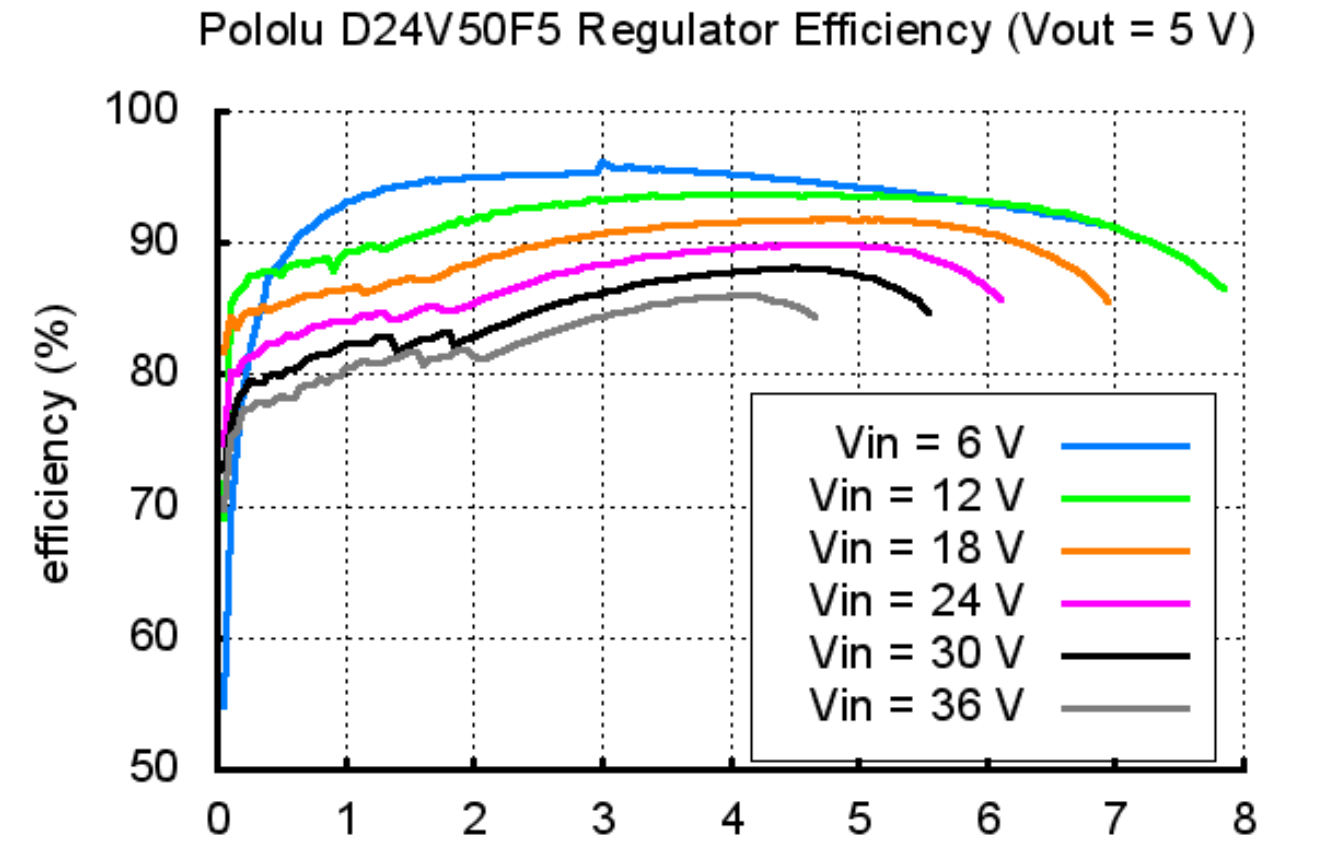
\includegraphics[width=0.4\textwidth]
	{resources/D24V50F5.PNG}
	\caption[Wirkungsgrad D24V50F5]{Wirkungsgrad D24V50F5 \protect\cite{D24V50F5}}
	\label{fig:D24V50F5}
\end{figure}

\subsection{Ethernet Schleifring}
\label{subsec:Schleifring}
Da übliche Kabel nur für einige wenige Verdrehungen ausgelegt sind und so bei drehenden Vorrichtungen kaputt gehen, wird ein Schleifring als Drehübertrager eingesetzt. Ein Schleifring überträgt das Eingangssignal über eine Bürste und bildet somit einen Gleitkontakt. Die Problematik liegt beim Velodyne VLP-16, dass die Datenübertragung über Ethernet übermittelt werden muss. Gängige Schleifringe bieten keine Gewähr für die Übertragung von Ethernet, da die Datenrate verhältnismässig hoch ist. Es gibt jedoch einige wenige Hersteller aus dem amerikanischen und asiatischen Markt, welche Ethernet-Übertrager vertreiben. Ein Ethernet-Schleifring, der zusätzlich Leistungsübertragungen bis 5 Ampere zulässt, kostet nach Abklärungen bei diversen Herstellern zwischen 120 - 600 Fr..

\subsection{Ethernet Switch}
\label{subsec:Ethernetswitch}
Die Einplatinencomputer aus Kapitel \ref{sec:Datenverarbeitung} benötigen mit Ausnahme des Up Board Squared ein weiteren Ethernetanschluss, damit die Kommunikation gewährleistet ist. Ethernet Switches gibt es in diversen Variationen und Grössen. Für die Aufgabenstellung wird ein möglichst kompakter Switch benötigt, der mindestens drei Anschlüsse bietet. Im Preissegment von 30 Fr. können bei Mouser, Distrelec und Farnell sehr kompakte 5-Port Switch bestellt werden. Eine gute Lösung ist dafür der Ethernet Switch GS105 der Marke Netgear. Dieser benötigt einen 12 Volt Speisung, mit dem sich eine Spannungsanpassung erübrigen würde. Zudem ist er im direkten Vergleich das Produkt mit den kleinsten Abmessungen.

\section{Zwischenfazit}
\label{ZwischenfazitInfo}
Für die Einarbeitung in das Projekt ist die Informationsbeschaffung bzw. Recherche ein wesentlicher Bestandteil. Dabei werden wichtige Grundlagen für die Konzeption geschaffen. ROS bietet für 3D-Mapping gute Tools und vereinfacht die Datenverarbeitung des Velodyne VLP-16 bedeutend. Mittels Schrittmotoren oder Gleichstrommotoren kann der Velodyne gedreht werden. Mit entsprechender Sensorik können damit die räumliche Messungen erfolgen. Für die Datenverarbeitung stehen mehrere Einplatinencomputer zur Verfügung, dabei müssen diese jedoch die Kriterien erfüllen. Für endlos drehende Vorrichtungen wird zusätzlich ein Ethernet Schleifring benötigt, da ansonsten die Kabelführung nicht gewährleistet ist.  

 \clearpage
\chapter{Konzeption}
\label{Konzeption}

\section{Blindtext}
\Blindtext[2][3] 


\section {Projektauftrag}
\label{eruierte_Komponenten}

\section{Zwischenfazit}
\label{Zwischenfazit_konzept}

\section{Ziele}
\blinditemize \clearpage
\chapter{Realisierung}
\label{chap:Realisierung}
Dieses Kapitel beschreibt die Realisierung des Prototyps. Der Prototyp ist eine überarbeitete Version der Konzeptvariante 2, siehe Unterkapitel \ref{sec:var2}. Es mussten Änderungen bei verschiedenen Komponenten durchgeführt werden, diese werden im Unterkapitel \ref{sec:mechKomp} erläutert. In Abbildung \ref{fig:Gesamtbild} ist das realisierte Konzept ersichtlich.

\begin{figure}[H]
	\centering
	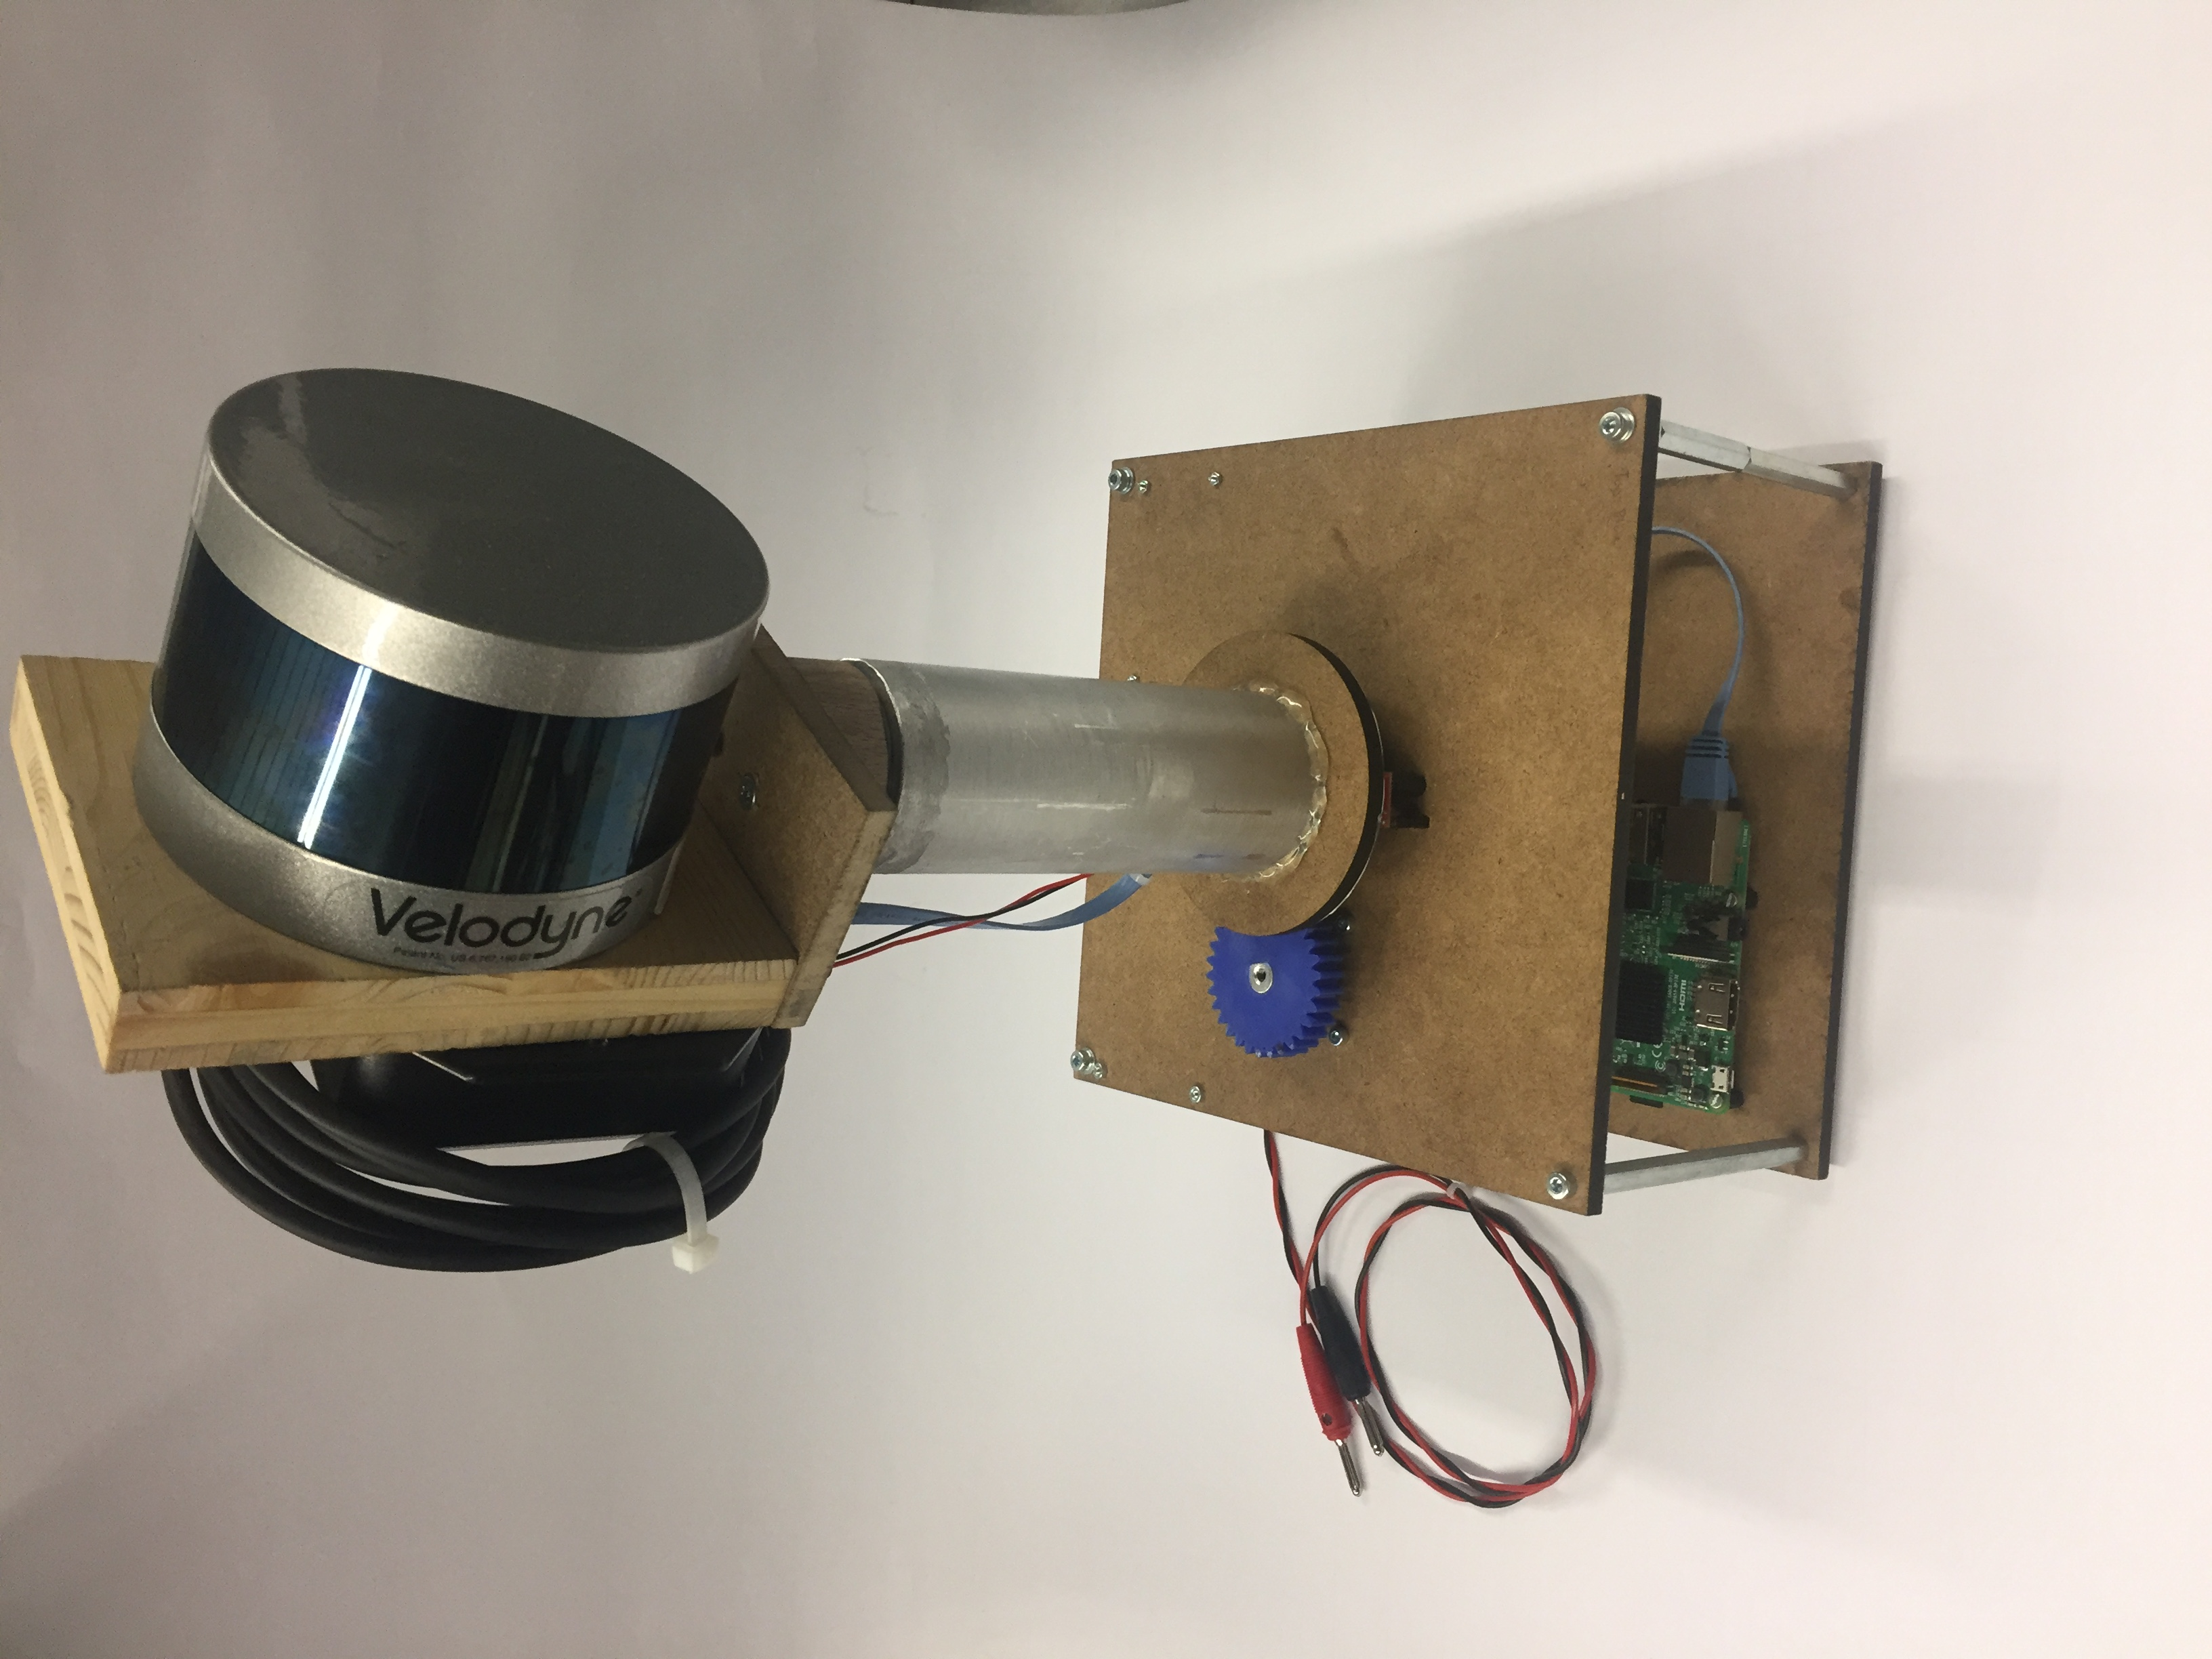
\includegraphics[angle=-90,width=0.58\textwidth]{resources/Gesamtbild.JPG}
	\caption[realisiertes Konzept]{realisiertes Konzept}
	\label{fig:Gesamtbild}
\end{figure} 


\section {Hardware}
\label{sec:Hardware}

Da beide Projekte, welche im Unterkapitel \ref{sec:Vorzeigeprojekte} eine endlos drehende Konstruktion nutzen, sowie die Aufgabenstellung im Anhang \ref{Pflichtenheft} eine drehende Konstruktion vorgibt, wurde eine endlos drehende mechanische Konstruktion angefertigt. 

\subsection {mechanische Komponenten \& Gehäuse}
\label{sec:mechKomp}

Um eine möglichst einfache und schnelle Lösung zu realisieren, wurden die mechanischen Komponenten nach Verfügbarkeit ausgewählt. Die Masse des Alurohrs und der Zahnräder waren größtenteils durch die verfügbare Grösse des Kugellagers gegeben. Das Kugellager wurde so gewählt, dass ein Ethernet RJ45 Stecker hindurchgeführt werden kann. Daraus ergibt sich einen Innendurchmesser von 22 mm und der entsprechende Aussendurchmesser von 44 mm.
Das Kugellager wurde direkt in das Alurohr gepresst und zusätzlich seitlich mit Schrauben verkeilt. Das Alurohr wurde mit einem Aussendurchmesser von 50 mm und einer Wandstärke von 3mm gewählt. Einerseits ist so der Innendurchmesser des Alurohrs passend zum Aussendurchmesser des Kugellagers und anderseits können bei dieser Wandstärke Gewinde geschnitten werden, damit Schrauben als Keil verschraubt werden können.

Der innere Ring des Kugellagers wurde auf den Kugellageradapter gesteckt. Dieser ist wiederum wie in Abbildung \ref{fig:mechKomp} an der Deckplatte befestigt. Somit lässt sich das Alurohr mit wenig Reibung drehen.

Die zwei Zanhräder wurden mit dem CAD-Tool OnShape gelayoutet und im FabLab mit einem 3D-Drucker erzeugt. Das grosse Zahnrad mit 48 Zähnen besitzt den Innendurchmesser 50 mm, welcher dem Alurohr entspricht. Dieses wurde auf das Alurohr gepresst. Das zweite Zahnrad ist im Verhältnis 1.5:1 kleiner und besitzt 32 Zähne. Die Übersetzung wurde so gewählt, dass die Komponenten mit genügend Abstand nebeneinander montiert werden können. Dieses Verhältnis muss bei der Softwareimplementierung berücksichtigt werden.

\begin{figure}[H]
	\centering
	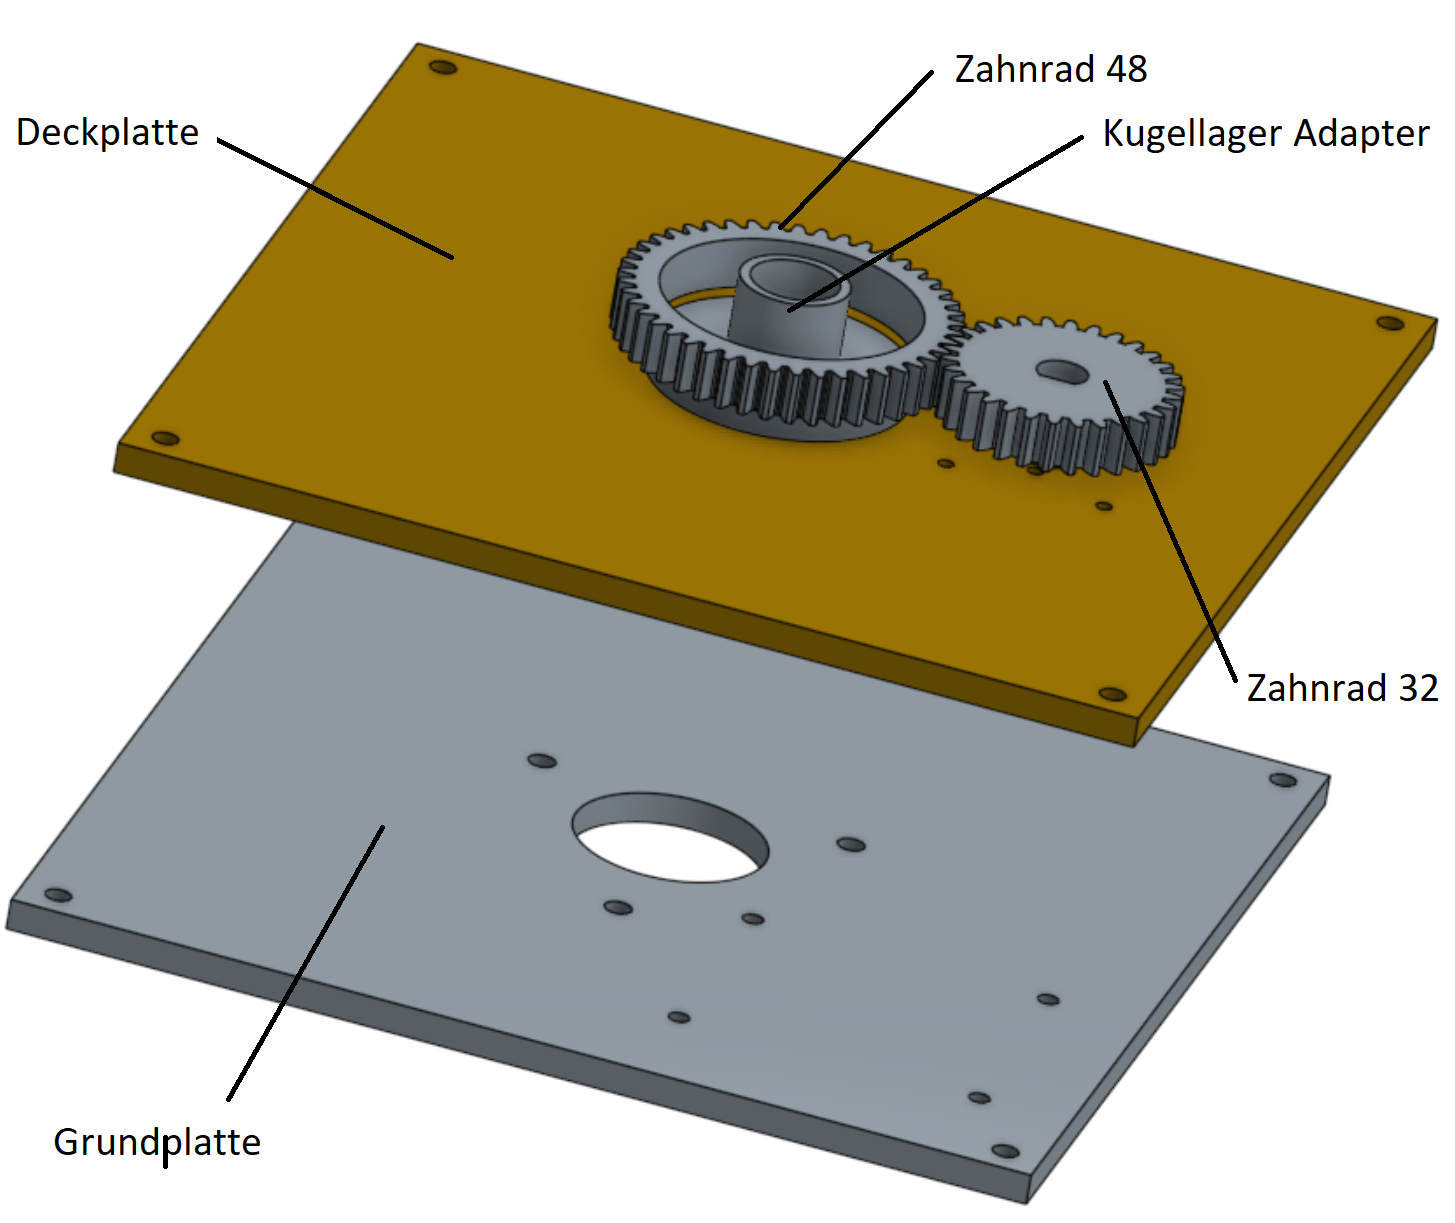
\includegraphics[width=0.8\textwidth]{resources/mechKomp2.PNG}
	\caption{gelayoutete Komponenten in OnShape}
	\label{fig:mechKomp}
\end{figure} 

Die Grösse der Platten wurde so gewählt, dass alle Komponenten dazwischen verbaut werden können. Daher wurden zwei MDF-Platten mit den Massen 200 mm x 200 mm x 6 mm (HxBxT) im FabLab erstellt. Die Grund- und Deckplatten wurden in OnShape gelayoutet und besitzen bereits vorgefertigte Löcher für die Montage der elektrischen Komponenten.

\subsection {elektrische Komponenten}
\label{sec:elekKomp}

Der Velodyne VLP-16 wurde auf einen rechtwinklige Konstruktion montiert, so dass der Lasermittelpunkt möglichst auf der Drehachse liegt. Die Interface Box wurde direkt gegenüber des Lasers montiert. Über den Schleifring führen eine 12 Volt Speisung und das Ethernetkabel direkt zu den erforderlichen Anschlüssen. Mit dieser Konfiguration lässt sich der Velodyne über die Zahnräder endlos drehen.

Die Nullposition wird mittels dem QRE 1113 und einem Hohlzylinder detektiert. Der Hohlzylinder ist dabei am rotierenden Alurohr befestigt. Der QRE 1113 ist mit dem Abstand von 2 mm unterhalb des Hohlzylinder fest montiert. Indem auf dem Hohlzylinder ein schwarzer Streifen auf eine weisse Oberfläche gedruckt ist, kann der Nullpunkt detektiert werden.

\begin{figure}[H]
	\centering
	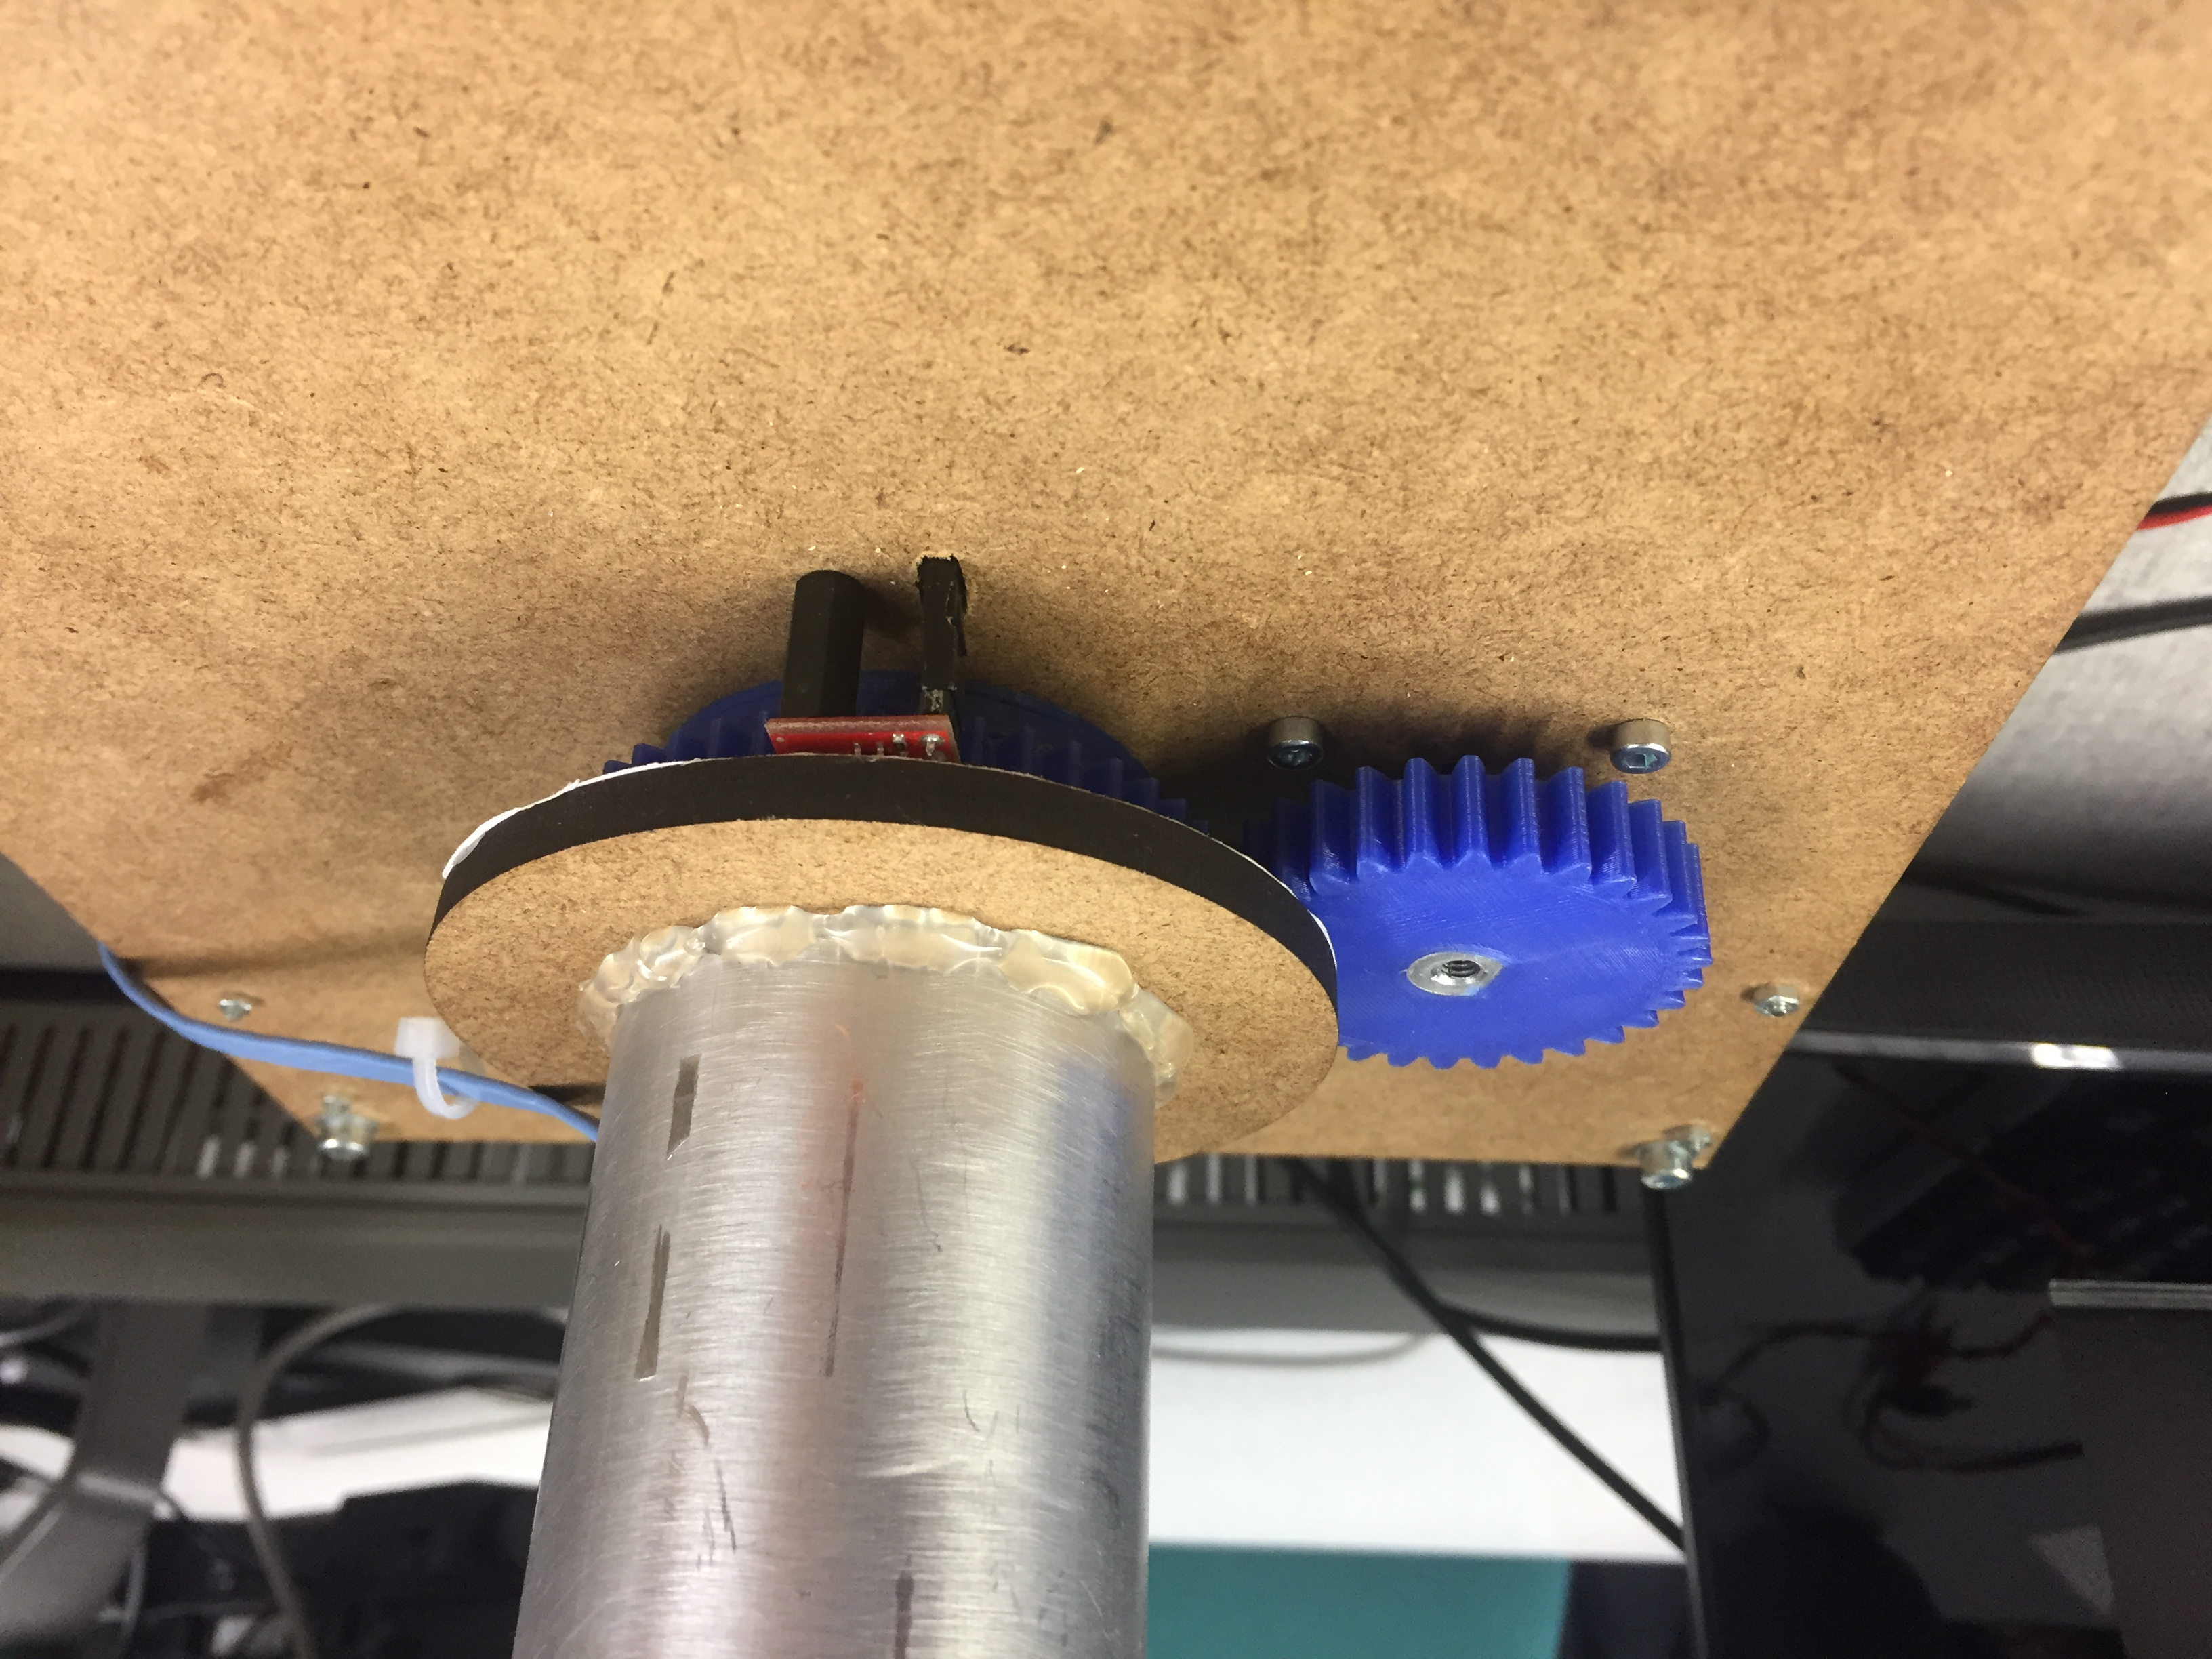
\includegraphics[angle=180,width=0.6\textwidth]{resources/Nullposition.jpg}
	\caption{Nullpunkterkennung mittels QRE 1113}
	\label{fig:Nullposition}
\end{figure} 

In der Konzeption wurde ein Gleichstrommotor der Marke Pololu für den Antrieb ausgewählt (siehe Unterkapitel \ref{subsec:Gleichstrommotor}). Während der Realisierung wurden sehr spät (Kalenderwoche 11) bedeutende Fehlverhalten des Motors festgestellt. Während den Leerlaufmessungen (Kalenderwoche 7) konnten keine Abweichungen der Encodersignale festgestellt werden. Nach dem Verbauen des Gleichstrommotors entsprachen die Encoder-Signale nicht den zu erwartenden Ergebnissen. Die Messwerte weichen mit bis zu 200 \ac{CPR}, welches umgerechnet ca. 36$^\circ$ ist vom Sollwert von 2248 ab. Dies verursacht unbrauchbare Resultate beim zusammenfügen der Punktwolken. Der Motor besitzt zusätzlich eine nicht nachvollziehbares Fehlverhalten. In einer Messung des Motorentreibers wurde ein fehlerfreies \ac{PWM} ausgemessen und auch die nötigen Strom- (1 Ampere) und Spannungswerte (12 Volt) verifiziert. Dennoch blockiert der Motor kurzzeitig willkürlich bei verschiedenen Drehpositionen. Dieses Fehlverhalten könnte auf ein internen Getriebedefekt zurück zu führen sein. Ursache für dieses Verhalten kann die Befestigungsschraube sein, welche bei der Montage hinein gedreht wurde. 

Aus den erwähnten Gründen wurde schnellst möglichst eine Alternative eruiert. Bei der Alternative handelt es sich um einen Schrittmotor der Marke Trinamic. Dieser Motor wurde aus Gründen der Verfügbarkeit und aus bereits bestehenden Kenntnissen über dessen Funktionsweise ausgewählt. Mit diesem Schrittmotor ist es möglich eine gleichmässige Umdrehungsgeschwindigkeit zu erreichen. 

Die Software wurde auf die neue Konfiguration angepasst und ist in Abschnitt \ref{subsec:Ansteuerung} erläutert. Es werden mittels 1/16 Schritte insgesamt 3200 Schritte für eine Umdrehung bei diesem Motor benötigt. Daraus ergibt sich mit der Übersetzung eine maximale Auflösung von $\frac{360^\circ}{1.5 * 3200}$ = 0.075$^\circ$. 
\todo{schrittverluste}

\section{Software}
\label{sec:SoftwareReal}
Wie bereits im Kapitel \ref{sec:Software} erläutert, wird durch das Velodyne Package ein grosser Teil der Aufgabenstellung bereits abstrahiert. Die einzelnen Aufgabenblöcke wurden nochmals unterteilt und sind in Abbildung \ref{fig:software_flow} dargestellt. Einerseits ist es nötig den Datenstream in einem weiteren Node zu empfangen und anderseits muss die Position ermittelt werden. Diese beiden Daten werden im Node \textit{/velodyne\_combined} zusammengefügt. Sobald die Daten kombiniert werden können, muss in einem weiteren Schritt die kombinierten Daten in einem Container gespeichert werden und bei Bedarf versendet.

\begin{figure}[H]
	\centering
	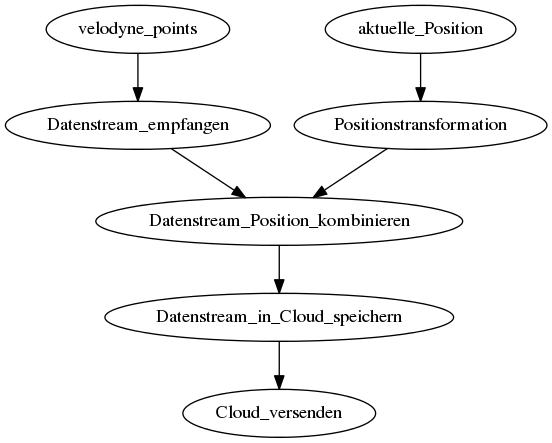
\includegraphics[width=0.5\textwidth]{resources/software_flow.png}
	\caption{Software Ablaufstruktur}
	\label{fig:software_flow}
\end{figure}  

Die Software wurde aufbauend konzipiert. Dabei wurde in einer ersten Phase das Empfangen und Weiterleiten mittels ROS \textit{Publisher und Subscriber} programmiert. In einem zweiten Schritt wurde die aktuelle Position mit den Daten kombiniert. In der letzte Phase wurde die Software mit dem Zusammenfügen der Datenpunkte zu einer Punktwolke erweitert. Wesentliche Codeausschnitte werden in den entsprechenden Unterkapiteln erläutert.

In Abbildung \ref{fig:rqt_graph_erweitert_2} ist mit \textcolor{red}{roter} Umrandung die Softwareerweiterung ersichtlich. Diese wurde in einem eigenen Package namens Laser\_3D erarbeitet, das im digitalen Anhang zu finden ist. 

\begin{figure}[H]
	\centering
	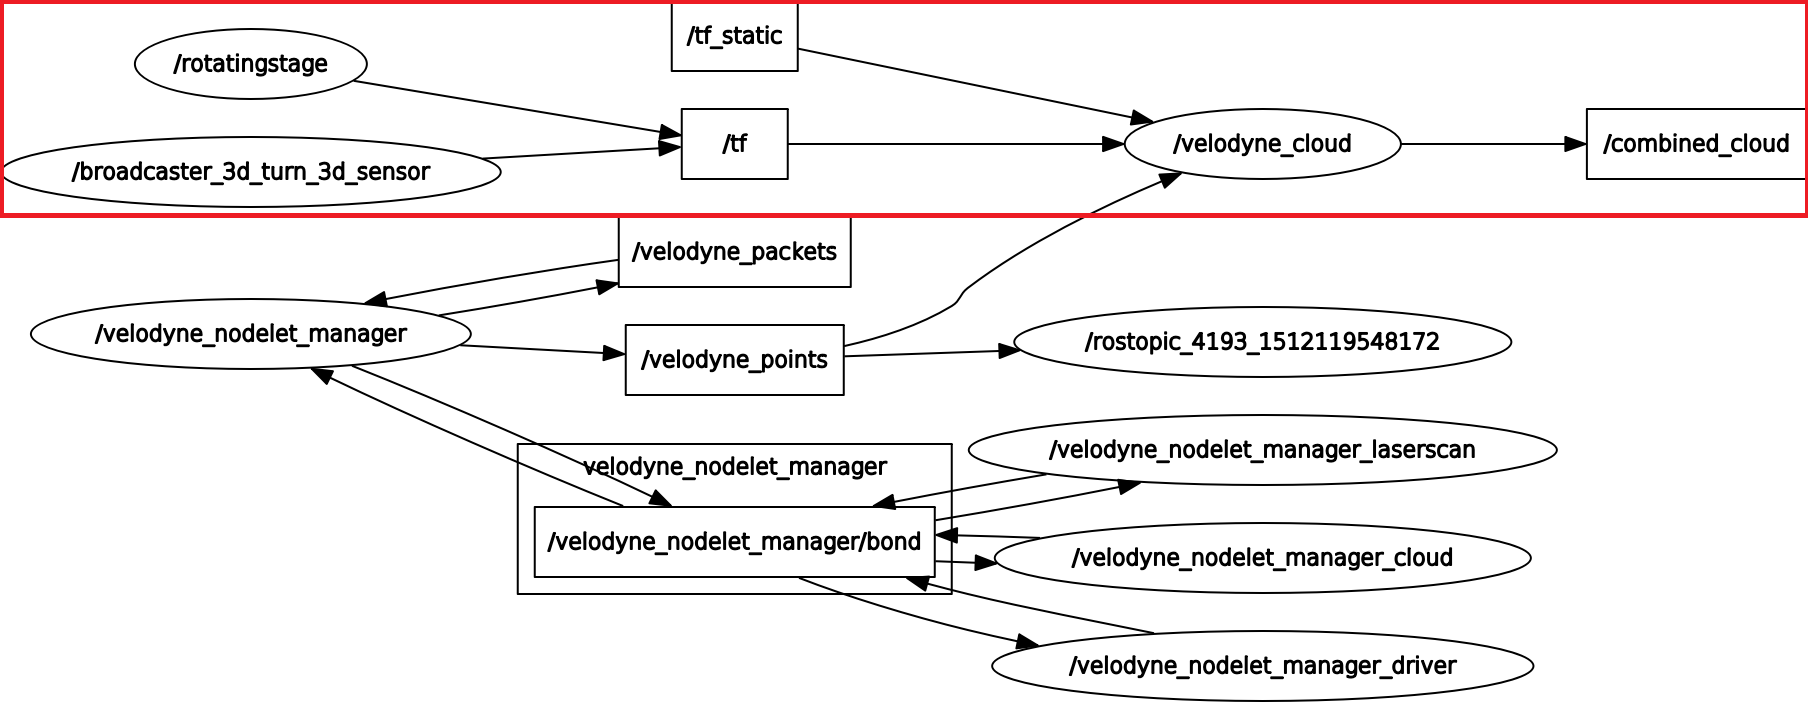
\includegraphics[width=0.75\textwidth]{resources/rqt_graph_erweitert_2.png}
	\caption{Softwareerweiterung mit Laser\_3D}
	\label{fig:rqt_graph_erweitert_2}
\end{figure} 
\subsection{Phase 1: Empfangen und Weitersenden}
\label{subsec:Phase2}
In dieser Phase wurden zu Beginn eine Programm implementiert, welche die Sensordaten (\textit{Messages}) empfängt und direkt wieder weiterleitet. Diese Funktion bietet das Grundgerüst für die weiteren Phasen. ROS bietet für diese Funtion zwei generische Klassen an. Der Publisher versendet Messages über sogenannte Topics, wie beispielsweise die \textit{velodyne\_points (vom Typ: velodyne\_msgs/PointCloud2)}. Subscriber können von Topics die Messages mittels einer Callback-Funktion an Variablen übergeben. Nachfolgend sind dazu die wesentlichsten Codeauschnitte wiedergegeben. \cite{pubsub} \todo{bilder schieben}

\begin{figure}[H]
	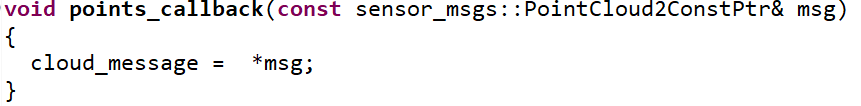
\includegraphics[width=0.62\textwidth]{resources/sourcecode/callback.png} \\
	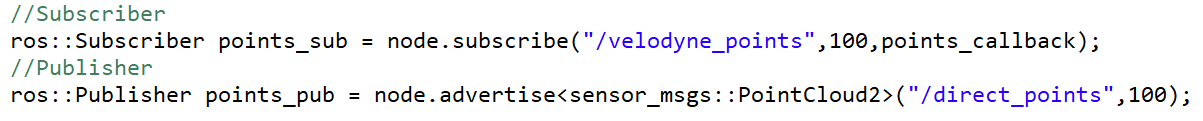
\includegraphics[width=0.9\textwidth]{resources/sourcecode/pubsub.png}
	%\caption{zusammengefügte mechanische Komponenten}
	\label{fig:pubsub}
\end{figure} 

\subsection{Phase 2: Positionstransformation}
\label{subsec:Phase}

Der empfangene Sensorstream kann mit Koordinatentransformation in die aktuelle Position des Drehturms transformiert werden. Es wird an dieser Stelle für die nachfolgenden Betrachtungen kurz Bezug zu Koordinatentransformation genommen \cite{Koordinaten}.
Es gelten für dreidimensionale Drehbewegungen folgende Matrizen:

$R_x(\phi ) =\begin{bmatrix}
	1&  0& 0\\ 
	0&  \cos\phi&  \sin\phi\\ 
	0&  -\sin\phi&  \cos\phi
\end{bmatrix}, R_y(\theta ) = \begin{bmatrix}
	\cos\theta&  0& -\sin\theta \\ 
	0&  1& 0\\ 
	\sin\theta &  0& \cos\theta 
\end{bmatrix}, R_z(\psi ) =\begin{bmatrix}
	\cos\psi& \sin\psi  & 0 \\ 
	-\sin\psi&  \cos\psi& 0 \\ 
	0&  0& 1
\end{bmatrix}$

Mit dem Rollwinkel $R_x(\phi)$ \textit{(engl. roll)}, Nickwinkel $R_y(\theta )$ \textit{(engl. pitch)} und Gierwinkel $R_y(\theta )$ \textit{(engl. yaw)} können in die 3 Freiheitsgrade beliebige Transformationen statisch oder dynamisch vorgenommen werden. Alternative können die Bewegungen mittels \ac{Quaternionen} angegeben werden. In Abbildung \ref{fig:rollpitchyaw} sind die Drehbewegungen mit den Achsen visualisiert.

\begin{figure}[H]
		\centering
	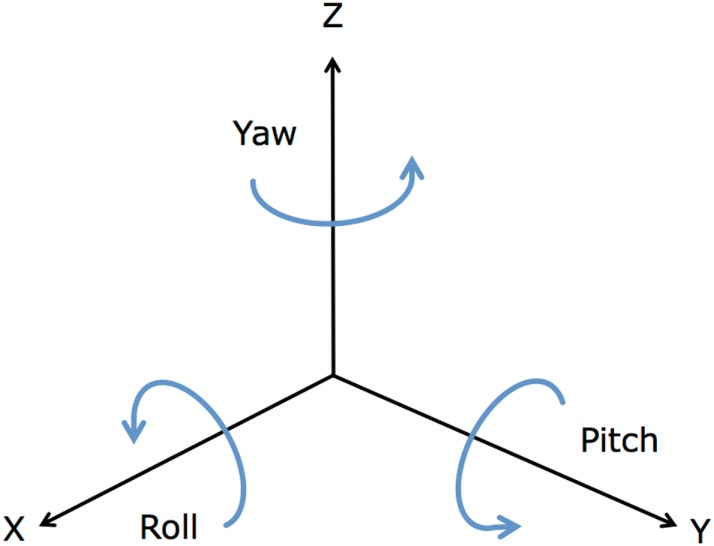
\includegraphics[width=0.3\textwidth]{resources/rollpitchyaw.png}
	\caption[{Roll-Pitch-Yaw mit X-Y-Z-Achsen}]{Roll-Pitch-Yaw mit X-Y-Z-Achsen}
	\label{fig:rollpitchyaw}
\end{figure} 

ROS bietet die Möglichkeit mehrere Koordinatensysteme miteinander zu verlinken und über die Klassen \textit{TF Broadcaster} und \textit{TF Listener} die aktuellen Positionen zu versenden und empfangen. In einem separaten Programmsegment \textit{rotatingstage} (siehe Abbildung \ref{fig:rqt_graph_erweitert_2}) wurde ein TF Broadcaster implementiert, welcher die aktuelle Ausrichtung des Drehturm versendet. Nachfolgender Codeauschnitte erläutern wesentliche Elemente. Es werden die Objekte \textit{TransformBroadcaster}, \textit{Transform} und \textit{Quaternion} verwendet, damit eine Bewegung erstellt wird.
\begin{figure}[H]
	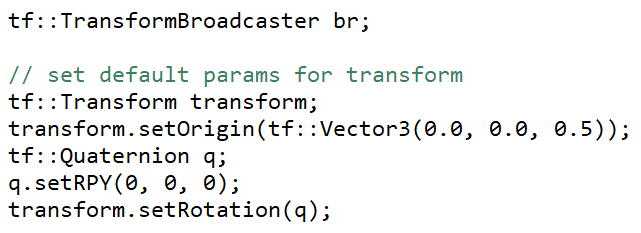
\includegraphics[width=0.5\textwidth]{resources/sourcecode/tf_broadcaster.png}	
\end{figure} 
Wird die aktuelle Position des Motors als Winkel phi übergeben und fortlaufend als Drehung in der Z-Achse (yaw) versendet, lassen sich die Koordinatenachsen verschieben. Da der Velodyne VLP-16 um -90$^\circ$ (270$^\circ$) geneigt ist, wurde die Transformation entsprechend gedreht (roll). Die versendete Transformation besitzt neben aktueller Position, einen Zeitstempel und die betreffenden Koordinatensysteme.
\begin{figure}[H]
	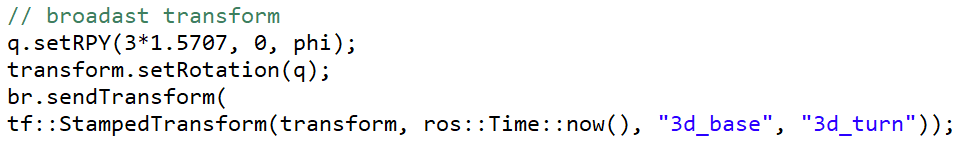
\includegraphics[width=0.8\textwidth]{resources/sourcecode/setrotation.png}	
\end{figure}
Der Node \textit{/velodyne\_combined} wurde mit einem TF Listener erweitert. Dieser ruft in einer lookup-Funktion die aktuelle Transformation ab und speichert diese in eine Variable.
\begin{figure}[H]
	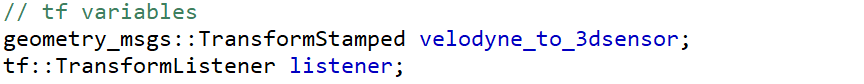
\includegraphics[width=0.7\textwidth]{resources/sourcecode/tf_listener.png}
	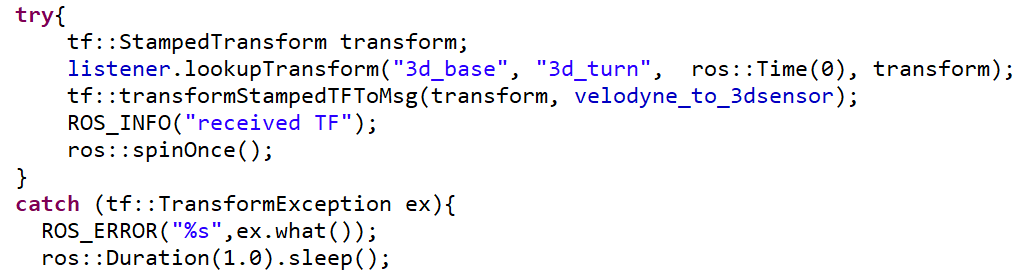
\includegraphics[width=0.7\textwidth]{resources/sourcecode/tf_update.png}		

\end{figure}
In Abbildung \ref{fig:koordinaten} sind die zwei Koordinatensysteme mit Rviz visualisiert. Die drehende Achse 3d\_turn, die mit der Achse 3d\_base verlinkt ist.
\begin{figure}[H]
	\centering
	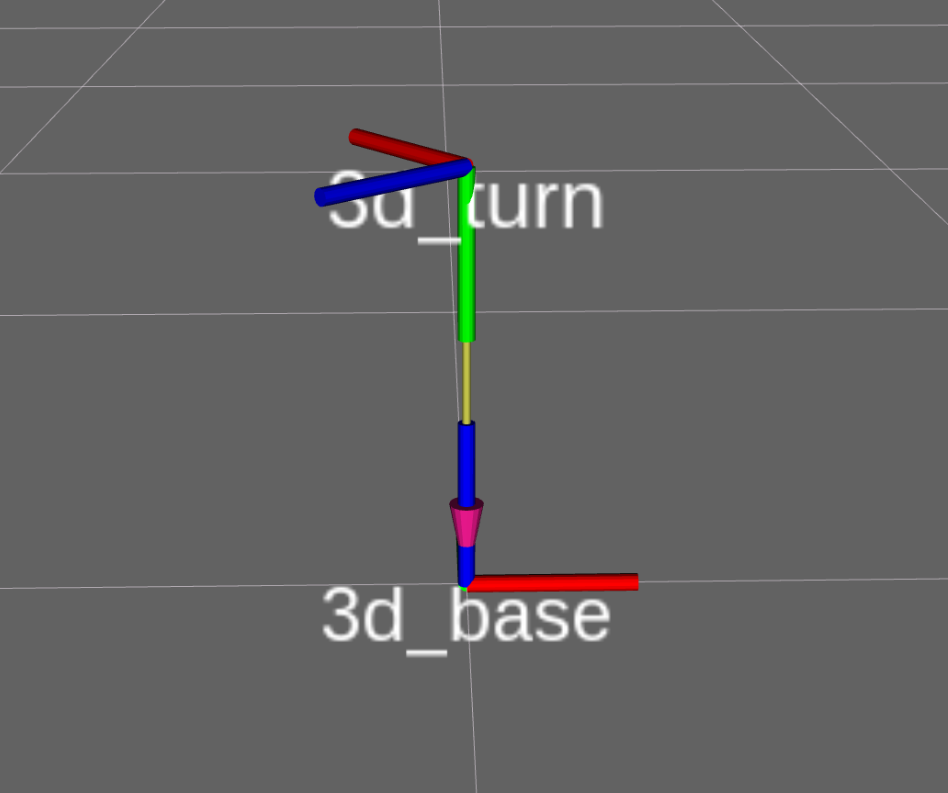
\includegraphics[width=0.5\textwidth]{resources/tf_rotation.PNG}
	\caption[dynamische Koordinatentransformation]{dynamische Koordinatensysteme}
	\label{fig:koordinaten}
\end{figure} 

\subsection{Phase 3: Punktwolke zusammenfügen}
\label{subsec:Phase3}
Während dieser Phase wurde eine \ac{Refactoring} gemacht und eine Klasse SubListener eingeführt. Ohne die Klasse verfügen mehrere Variablen nicht über den nötigen \ac{Scope}. In folgender Abbildung ist das Klassendiagramm mit entsprechenden Funktionen ersichtlich.

\begin{figure}[H]
	\centering
	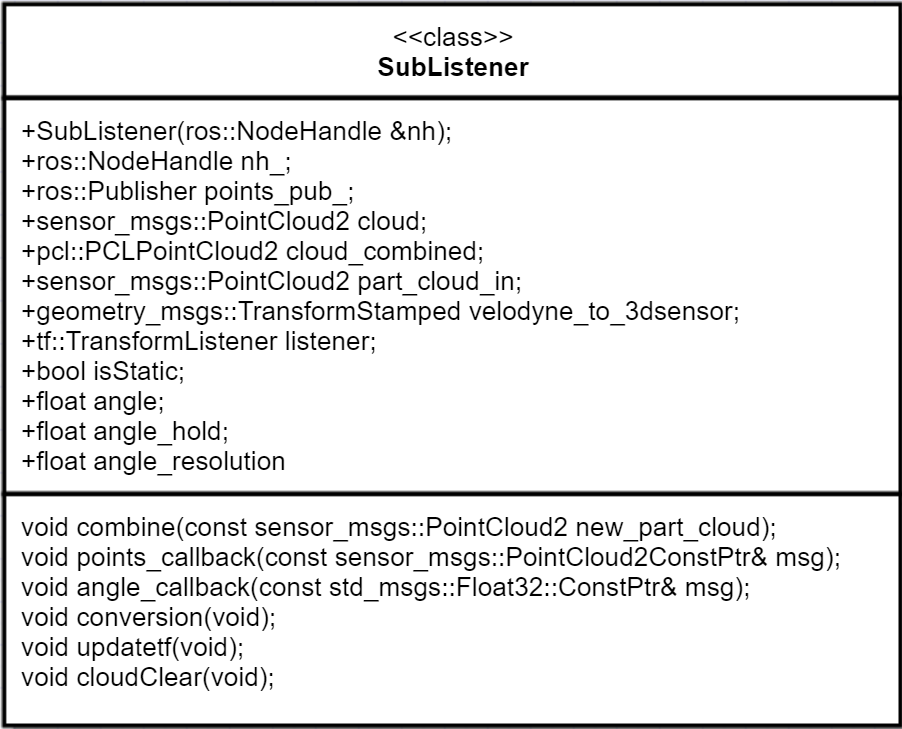
\includegraphics[width=0.5\textwidth]{resources/classdiagram.PNG}
	\caption[UML Klassendiagramm SuListener]{UML Klassendiagramm SubListener}
	\label{fig:classSubListener}
\end{figure} 

Die Klasse regelt alle Funktionen für das zusammenfügen der Punktwolken. Auf die detaillierte Erläuterungen wird in diesem Abschnitt verzichtet. 



In Abbildung \ref{fig:pointcloud_test} ist ein zusammengefügte Punktwolke ersichtlich. Durch entsprechende Parameteränderung lässt sich die Abtastung bei gegebener Umdrehungsgeschwindigkeit verändern.
 
\begin{figure}[H]
\centering
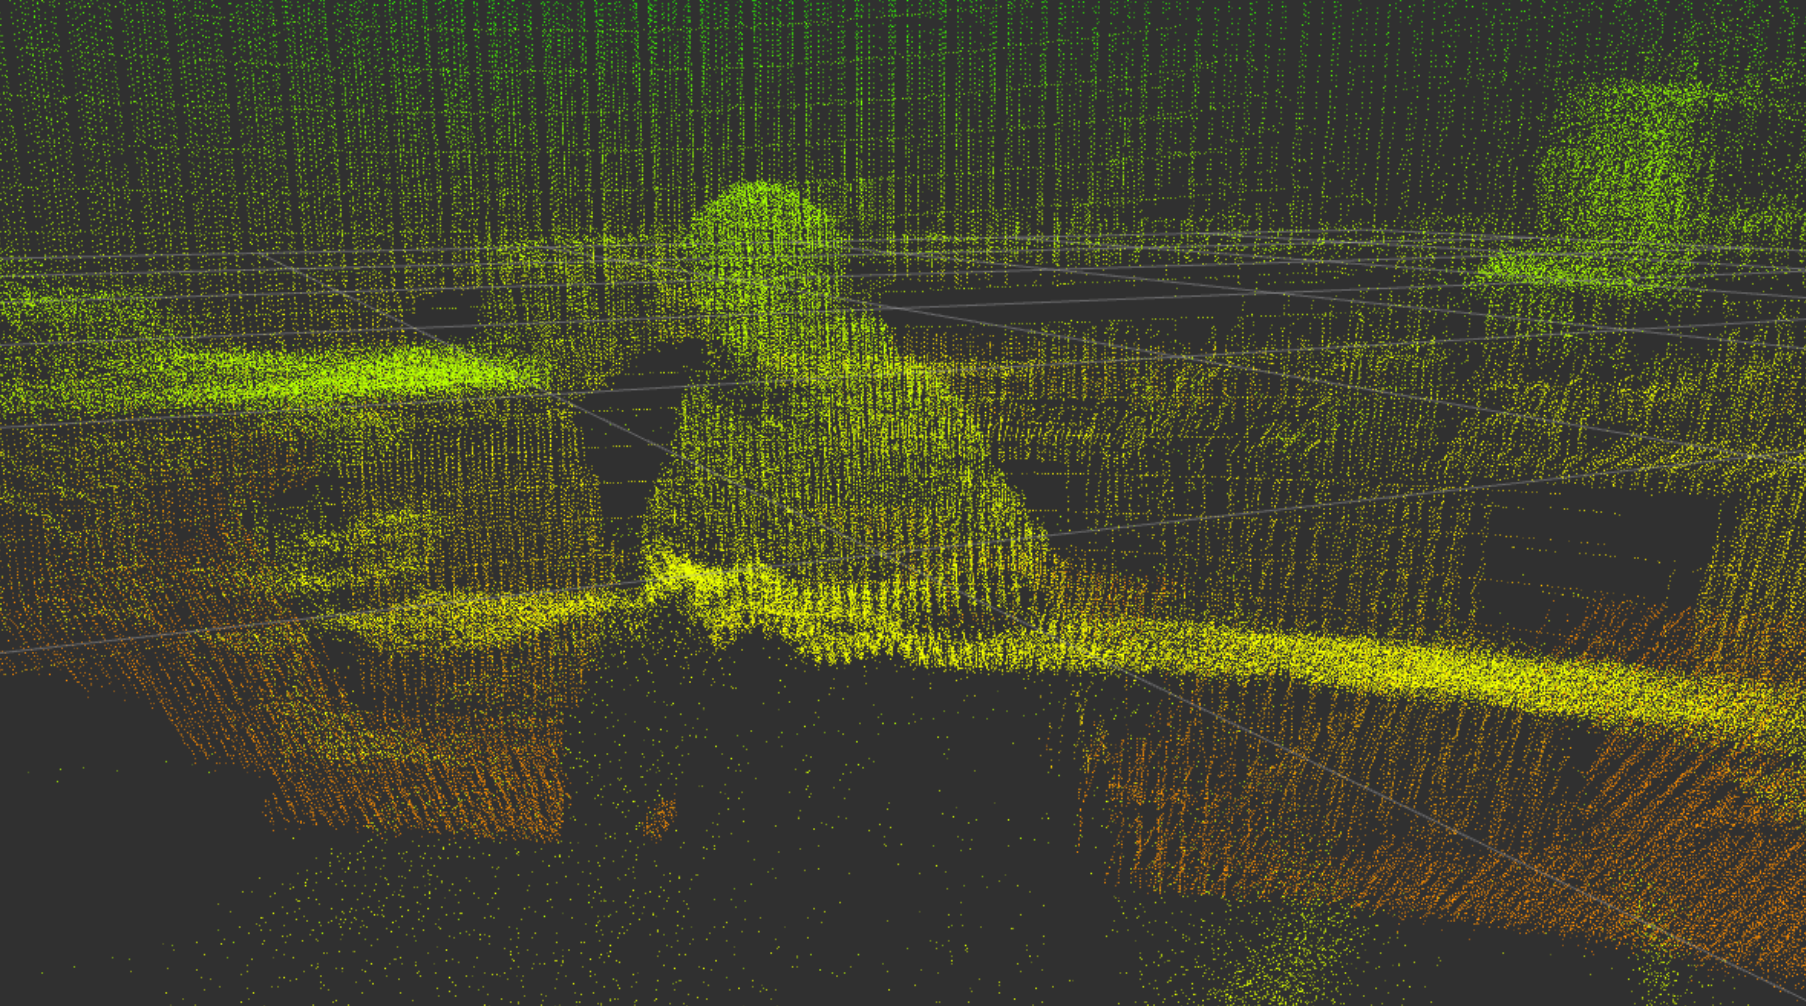
\includegraphics[width=1.0\textwidth]{resources/pointcloud_test.png}
\caption[Punktwolke einer Person bei Distanz 1m]{Punktwolke einer Person bei Distanz 1m}
\label{fig:pointcloud_test}
\end{figure}



In Abbildung \ref{fig:raumausmessung} ist ein Gesamtbild einer Punktwolke eines Raumes der Grösse 3 m x 15 m x 10m (HxBxT) ersichtlich. Die Abbildung zeigt die 

\begin{figure}[H]
	\centering
	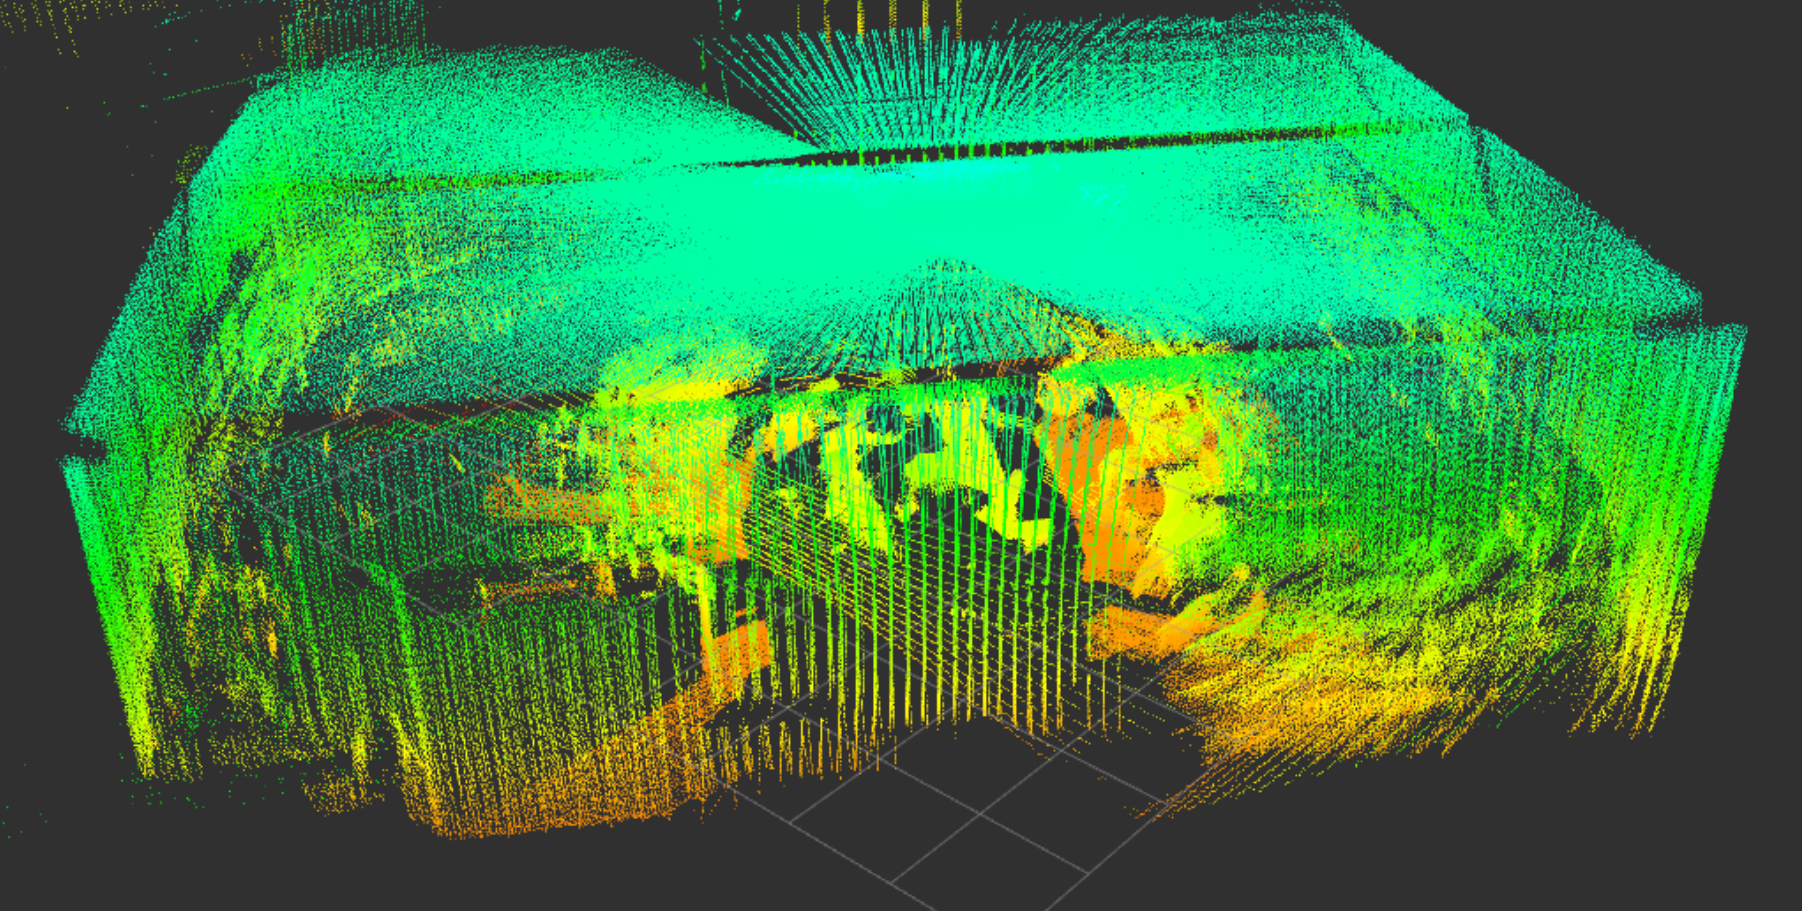
\includegraphics[width=1.0\textwidth]{resources/raumausmessung.png}
	\caption[zusammengefügte Punktwolken]{zusammengefügte Punktwolken}
	\label{fig:raumausmessung}
\end{figure}  



\subsection {Ansteuerung mittels GPIO}
\label{subsec:Ansteuerung}
\todo{gpio nach oben nehmen}
Wie bereits erwähnt wurde ein Schrittmotor der Marke Trinamic verwendet. Dieser wird über einen Motorentreiber A4988  angesteuert. Der Motorentreiber besitzt 


\section{Zwischenfazit}
\label{sec:ZwischenfazitReal}
ROS bietet viele Packages und Klassen, welche nützlich für die Softwareimplementation von Koordinatentransformation und Punktwolken sind. Die Freiheit von Open-Source bietet jedoch auch das Problem, dass die Kompatibilität von Packages nicht immer gewährleistet sind.  Anfänglich waren nru wenig Kenntnisse über die Koordinatentransformation vorhanden, daher verzögerte sich diese Softwarephase 2 erheblich. Es mussten einerseits die theoretischen Grundlagen verstanden werden und entsprechende Packages dazu evaluiert werden. Aufgrund z


 \clearpage
\chapter{Tests}
\label{chap:Tests}

\section{Testprotokolle}
\label{sec:Testprotokolle}
\Blindtext[2][3] 
\blinditemize

\section {Testergebnisse}
\label{sec:Testergebnisse}

\section{Fazit}
\label{sec:Fazit} \clearpage
\chapter{Reflektion}
\label{chap:Reflektion}

Die Aufgabenstellung konnte während der zur Verfügung stehenden Zeit nicht erfüllt werden. In den nachfolgenden Unterkapiteln wird Stellung genommen, aus welchen Gründen die definierten Ziele nicht erreicht wurden. Im Fazit werden Ergebnisse und Ziele gegenübergestellt und offene Punkte erläutert. Danach werden zum Projektmanagment einzelne Punkte aufgelistet mti Bezug zur detaillierten Projektplanung in Anhang \ref{Projektmanagment}. Der Ausblick bietet Aufschluss, welche weiteren Tätigkeiten zur Erfüllung der Aufgabenstellung geführt hätten. Zuletzt wird im Schlusswort eine persönliches Resümee gemacht.
\section{Fazit}
\label{sec:}

\section{Erläuterungen Projektmanagment}
\label{sec: pm}

Die Projektplanung wurde in der KW  aufgegliedert. Dabei gab es einige bedeutende Arbeitspakete, welche das Projektmanagment stark beinflusst haben. Die Einschätzung des zeitlichen Aufwands für die Erstellung der Software wurde falsch bewertet. Es musste bedeutend mehr Zeit für die Softwareentwicklung aufgewendet werden. Dies hat einerseits mit den ungenügenden Kenntnissen über die Programmiersprache C++ und dem Framework ROS zu tun. Anderseits konnten  Mehrere ROS-spezifische Fehlermeldungen, welche nur durch die Unterstürzung von Herr Jensen behoben werden konnten, nahmen viel Zeit in Anspruch.


\section{Ausblick}
\label{sec: Ausblick}

Für diese Aufgabenstellung 

\section{Schlusswort}
Aus persönlicher Sicht bin ich mit der geleisteten Arbeit zufrieden. Ich kann aus dieser Industriearbeit sehr viele positive Erkenntnisse herausziehen und werde diese in Hinsicht auf die nächste Arbeit einfliessen lassen. Das zeitliche Fortschreiten in der Realisierungsphase und einige Fehlüberlegungen führten zu einem nicht vollständigen Produkt.  

\section{Danksagung}
An dieser Stelle möchte ich mir herzlich bedanken, die mich bei der Anfertigung dieser Arbeit unterstützt haben.

Zuallererst gebührt der Dank an Dr. Björn Jensen, der mich bei dieser Industriearbeit tatkräftige unterstützt hat, sowie mit wertvollen Hinweisen und schnellen Rückmeldungen zur Seite gestanden ist.
Mein Dank geht auch an Jonas Räber, der mir eine grosse Hilfe für die Einarbeitung mit \ac{ROS} war. Ebenfalls bedanken möchte ich mich bei den zwei Gegenleser Andreas Zimmermann und Angela Burch für die textuelle und inhaltliche Analyse der Dokumentation.

Zuletzt noch besten Dank and D 

 \clearpage
%\chapter{Beispiele} \label{c:beispiele}


Im Kapitel Beispiele (siehe \autoref{c:beispiele}) werden die möglichen Funktionen und\index{und} Möglichkeiten dies LaTeX-Dokuments demonstriert.

\section{Quelltext}

Nachfolgend der \autoref{lst:helloworld}.

\begin{lstlisting}[caption={Hello World}, captionpos=b, label={lst:helloworld}]
/**
* The HelloWorldApp class implements an application that
* simply prints "Hello World!" to standard output.
*/
class HelloWorldApp {
	public static void main(String[] args) {
		System.out.println("Hello World!"); // Display the string.
	}
}
\end{lstlisting}

\section{Bild}

\begin{wrapfigure}{R}{0.5\textwidth}
	\centering
	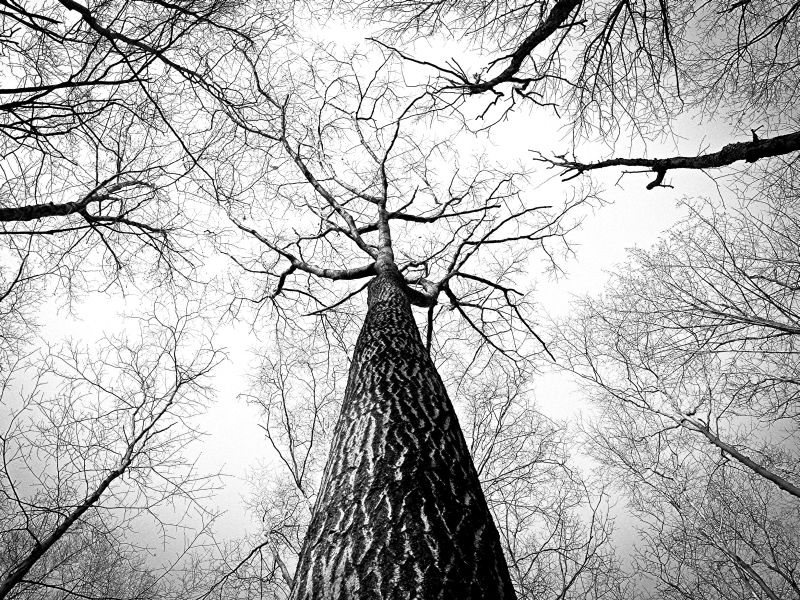
\includegraphics[width=0.5\textwidth]{resources/example}
	\caption{Beispielbild {\cite{PEXELS2015}}}
\end{wrapfigure}

Die rechts zu sehende Grafik demonstriert die Möglichkeiten des Paketes \glqq wrapfig\grqq . Grafiken innerhalb einer \glqq wrapfigure\grqq{} können entweder links oder rechts von Text umlaufen werden.


\section{Text Formatierungen und sonstiges}
Dieser Text enthält eine Fußnote\footnote{Fußnoten sind Anmerkungen, die im Druck-Layout aus dem Fließtext ausgelagert werden, um den Text flüssig lesbar zu gestalten.}.

\subsection{Listen}
Listen könne sowohl mit Bullet points als auch mit Zahlen erstellt werden
\begin{itemize}
	\item Eine Liste mit Bullet points
	\item Ein weiteres Element
\end{itemize}

\begin{enumerate}
	\item Eine Liste mit Zahlen
	\item Ein weiteres Element
\end{enumerate}

\subsection{Text Hervorhebungen}
\begin{quote}
	The problem with internet quotes is that you can't always depend on their accuracy \par\raggedleft--- \textup{Abraham Lincoln, 1864}
\end{quote}

"Inspirierende Zitate können mit epigraph eingefügt werden
\epigraph{The problem with internet quotes is that you can't always depend on their accuracy}{Abraham Lincoln, 1864}

Seitenumbrüche können nur direkt nach Text geschrieben werden, sonst lässt sich das Latex nicht mehr compilieren.
\\

\begin{figure}[H]
	\centering
	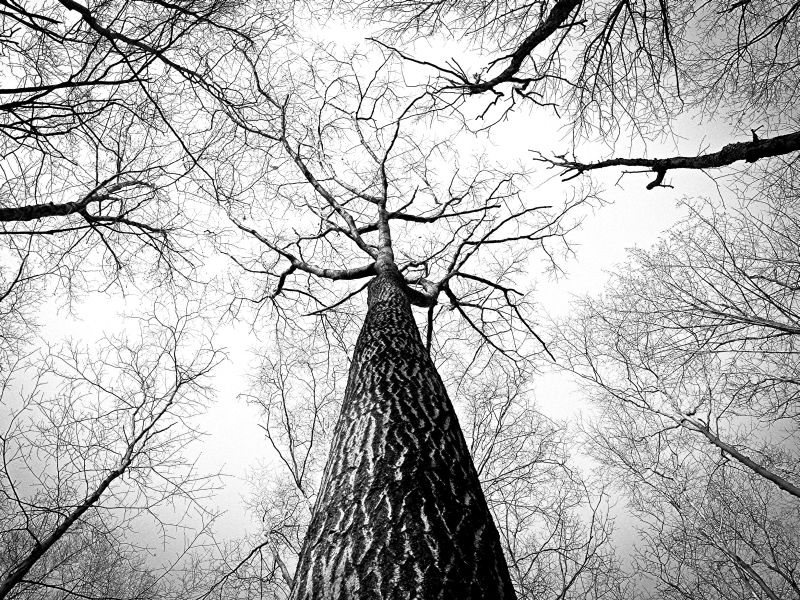
\includegraphics[width=0.7\textwidth]{resources/example}
	\caption{Beispielbild {\cite{PEXELS2015}}}
	\label{img:beispielbild}
\end{figure}

\section{Tabelle}

Nachfolgend \autoref{tbl:DigitalesZertifikat}.

\begin{table}[H]
	\begin{center}
		\renewcommand{\arraystretch}{1.3}
		\begin{tabular}{|l|}
			\hline
			\textbf{Inhaber:}\\
			Alice \\ \hline
			\textbf{Peer (Ersteller):}\\
			Bob \\ \hline
			\textbf{Öffentlicher Schlüssel des Inhabers:}\\
			F2 D2 0E ED FA 4E 9E 0A F2 DD 23 8A 32 44 F3 E9 \\ \hline
			\textbf{Gültigkeit:}\\
			2015-07-01 – 2016-06-30 \\ \hline
		\end{tabular}
	\end{center}
	\caption{Digitales Zertifikat}
	\label{tbl:DigitalesZertifikat}
\end{table}

\section{Long-Table}

Die \glqq Long-Table\grqq kann über definierte Header und Footer über Seitenumbrüche hinweg angezeigt werden.

\begin{longtable}{|l|l|l|l|}
	\hline
	\multicolumn{1}{|c}{\textbf{Version}} & \multicolumn{1}{|c}{\textbf{Codename}} &
	\multicolumn{1}{|c}{\textbf{API}} &
	\multicolumn{1}{|c|}{\textbf{Verteilung}} \\ \hline
	\endfirsthead
	
	\multicolumn{4}{c}{Fortsetzung - Verteilung der Androidversionen (Stand 01.02.2016)}\\ \hline
	\multicolumn{1}{|c}{\textbf{Version}} & \multicolumn{1}{|c}{\textbf{Codename}} &
	\multicolumn{1}{|c}{\textbf{API}} &
	\multicolumn{1}{|c|}{\textbf{Verteilung}} \\ \hline 
	\endhead
	
	\multicolumn{4}{c}{Fortsetzung auf nachfolgender Seite}
	\endfoot
	
	\caption{Verteilung der Androidversionen (Stand: 01.02.2016)}
	\label{tab:androidverteilung}
	\endlastfoot
	
	2.2 & Froyo & 8 & 0.1\%\\ \hline
	2.3.3 - 2.3.7 & Gingerbread & 10 & 2.7\%\\ \hline
	4.0.3 - 4.0.4 & Ice Cream Sandwich & 15 & 2.5\%\\ \hline
	4.1.x & Jelly Bean & 16 & 8.8\%\\ \cline{1-1} \cline{3-4}
	4.2.x &  & 17 & 11.7\%\\ \cline{1-1} \cline{3-4}
	4.3 &  & 18 & 3.4\%\\ \hline
	4.4 & KitKat & 19 & 35.5\%\\ \hline
	5.0 & Lollipop & 21 & 17.0\%\\ \cline{1-1} \cline{3-4}
	5.1 &  & 22 & 17.1\%\\ \hline
	6.0 & Marshmallow & 23 & 1.2\%\\ \hline
\end{longtable}

\section{Literaturverweis}

Weil für die alte\index{alte} und die neue Rechtschreibung verschiedene Trennregeln\index{Trennregeln} gelten, sind Deutsch mit alter Rechtschreibung und Deutsch mit neuer Rechtschreibung zwei verschiedene Sprachen (\cite{Knappen2009}, S. 192).

\section{Onlineverweise}

Siehe Google.de \cite{Google2015}.

\section{Glossar}




\section{Abkürzungsverzeichnis}


%\nomenclature{UGC}{User Generated Content}



 \clearpage
\input{chapter/Software} \clearpage

\pagenumbering{Roman}
\listoffigures \clearpage
\listoftables \clearpage
\lstlistoflistings \clearpage
\newpage
\fancyhead[L]{\nouppercase{Glossar}} %Kopfzeile links
\markright{GLOSSAR}
\chapter*{Glossar}\addcontentsline{toc}{chapter}{Glossar}
\begin{acronym}[LAMS aaaaaaaaa]
	  \acro{ARM}{Acorn Risc Machine}						\\	\acroextra{verbreitetes Mikroprozessor-Design, das grösstenteils auf 32Bit-Prozessoren beruht(ARMv7)}
	  \acro{AMD64}{X64}										\\	\acroextra{Prozessor-Architektur der handelsüblichen 64-Bit-PCs und Server}
 	  \acro{BSD}{Berkley Software Distribution}   			\\ \acroextra{frei verwendbare Lizenz, auch als Vorlage für kommerzielle Produkte}
 	  \acro{CPR}{Counts Per Revolution}						\\ \acroextra{}
 	  \acro{eMMC}{embedded Multimedia Card}   	 			\\ \acroextra{Digitales Speichermedium, basiert auf dem Prinzip der Flash Speicherung arbeitet}
  	  \acro{EnRicH}{European Robotic Hackathon}   	 		\\ \acroextra{weltweit erste und einzige Robotik Wettbewerb mit realen Szenarios}
 	  \acro{GPS}{Global Positioning System}      			\\ \acroextra{globales Navigationssatellitensystem zur Positionsbestimmung}
 	  \acro{GPU}{Grafikprozessor}				 			\\ \acroextra{spezialisierter Prozessor für Grafikanwendungen}
 	  \acro{IMU}{Inertiale Messeinheit}      				\\ \acroextra{Kombination mehrerer Trägheitssensoren}
      \acro{LIDAR}{Light Detection And Ranging}			 	\\ \acroextra{Verfahren zur optischen Distanzmessung}
      \acro{Mikrostepping}{Schrittteilung}					\\ \acroextra{Unteteilung der zu tätigenden Schritten bie Schrittmotoren um feinere Abstufungen zu erhalten}
      \acro{PCL}{Point Cloud Library}						\\ \acroextra{umfangreiche Softwarebibliothek für 3D Visualisierungen}
      \acro{KO}{Kathodenoszilloskop}		 				\\	\acroextra{Messgerät zur Analyse von Signalen}
      \acro{PWM}{Pulsweitenmodulation}						 \\ \acroextra{Modulationsverfahren mit varierenden Rechteckimpulsen}
      \acro{Quaternionen}{Erweiterung der komplexen Zahlen}								\\ \acroextra{Beschreibung von Drehbewegungen, bietet den Vorteil von eindeutigen 3D Positionen}
      \acro{RAM}{Random Acceess Memory}						\\ \acroextra{direkt ansprechbare Speicherbausteine}
      \acro{Refactoring}{ Strukturverbesserung}				\\ strukturelle Anpassung, verbessert Lesbarkeit, Wartbarkeit und Erweiterbarkeit
      \acro{ROS}{Robot Operating System}					\\ \acroextra{Software Framework für Robotikanwendungen}
      \acro{Scope}{Sichbarkeitsbereich}						\\ \acroextra{Sichtbarkeitsbereich einer Variable in einem Softwareprojekt}
      \acro{SD}{Secure Disk Memory Card}					\\ \acroextra{digitales Speichermedium, das nach dem Prinzip der Flash-Speicherung arbeitet}
      \acro{SOC}{Sysem-on-a-Chip}						 	\\ \acroextra{Integration der Funktionen eines programmierbaren elektronischen Systems auf einem Chip}
      \acro{State-Machine}{sequenzielle Ablauffolge}		\\ \acroextra{Verhaltensmodell einer Software, dass Aktionen, Zuständen und Zusandsänderungen beschreibt}
       \acro{UDP}{User Data Protocol}						\\ \acroextra{verbindungsloses Netzwerkprotokoll zur Versendung von Datagrammen von IP-basierten Rechennetzen} 
        \acro{XPC}{Barebone PC}								\\ \acroextra{kompakte unvollständige Computerdesign, meist mit vielen Schnittstellen und guter Erweiterbarkeit}
      
\end{acronym} 



%\printglossary[title={Glossar}] \clearpage
%\printglossary[style=dottedlocations,type=\acronymtype,title={Abkürzungsverzeichnis}] \clearpage

\printbibliography[heading=bibintoc, keyword={book}, title={Literaturverzeichnis}]\clearpage
\printbibliography[heading=bibintoc, keyword={online}, title={Onlinequellen}]\clearpage
\printbibliography[heading=bibintoc, keyword={image}, title={Bildquellen}]\clearpage

% Anhang
\fancyhead[L]{\nouppercase{\leftmark}} %Kopfzeile links
\appendix

\chapter{}
\addcontentsline{toc}{chapter}{Anhang A}

\section{Diagramm}

\section{Tabelle}

\section{Screenshot}

\section{Graph}

\end{document}